% demo.tex
%
% Enjoy, evolve, and share!
%
% Compile it as follows:
%   latexmk
%
% Check file `dithesis.cls' for other configuration options.
%
\documentclass[preface]{dithesis}

%\usepackage{graphicx}

%%%%%%%%%%%%%%%%%%%%%%%%%%%%%%%%%%%%%%%%%%%%%%%%%%%%%%%%%%%%%%%%%%%%%%%%%%%%%%%
%%%%%%%%%%%%%%%%%%%% User-specific package inclusions %%%%%%%%%%%%%%%%%%%%%%%%%
%%%%%%%%%%%%%%%%%%%%%%%%%%%%%%%%%%%%%%%%%%%%%%%%%%%%%%%%%%%%%%%%%%%%%%%%%%%%%%%
\usepackage{booktabs}
\usepackage{hyperref}
\usepackage{lipsum}
\usepackage{enumerate}
\usepackage{amsmath}
\usepackage{amssymb}

\usepackage{multirow}

\hypersetup{
    unicode=true,                     % non-Latin characters in bookmarks
    pdffitwindow=true,                % page fit to window when opened
    pdfnewwindow=true,                % links in new window
    pdfkeywords={},                   % list of keywords
    colorlinks=true,                  % false: boxed links; true: colored links
    linkcolor=black,                  % color of internal links
    citecolor=black,                  % color of links to bibliography
    filecolor=black,                  % color of file links
    urlcolor=black,                   % color of external links
    pdftitle={},                      % title
    pdfauthor={},                     % author
    pdfsubject={}                     % subject of the document
}
%%%%%%%%%%%%%%%%%%%%%%%%%%%%%%%%%%%%%%%%%%%%%%%%%%%%%%%%%%%%%%%%%%%%%%%%%%%%%%%
%%%%%%%%%%%%%%%%%%%% User-specific package inclusions %%%%%%%%%%%%%%%%%%%%%%%%%
%%%%%%%%%%%%%%%%%%%%%%%%%%%%%%%%%%%%%%%%%%%%%%%%%%%%%%%%%%%%%%%%%%%%%%%%%%%%%%%

\usepackage[colorinlistoftodos,bordercolor=orange,backgroundcolor=orange!20,linecolor=orange,textsize=scriptsize]{todonotes}
\newcommand{\kelly}[1]{\todo[inline]{\textbf{Kelly: }#1}} 
\newcommand{\ad}[1]{\textcolor{red}{#1}}
\newcommand{\aritra}[1]{\todo[inline]{\textbf{Aritra: }#1}} 


% \usepackage{algorithm}
% \usepackage{algorithmic}
% \usepackage[noend]{algpseudocode}
% \usepackage[ruled,vlined,linesnumbered]{algorithm2e}
% \SetAlFnt{\small}
\usepackage[ruled,vlined]{algorithm2e}
\usepackage{enumitem}

% \usepackage{verbatim}
%%% Basic sets
\newcommand{\R}{\mathbb{R}} % Reals
\newcommand{\N}{\mathbb{N}} % Naturals
\newcommand{\mbE}{\mathbb{E}} % Eucliden
\newcommand{\mcC}{\mathbb{C}} %continuous function
% caligraphic
\newcommand{\cA}{{\cal A}}
\newcommand{\cB}{{\cal B}}
\newcommand{\cC}{{\cal C}}
\newcommand{\cD}{{\cal D}}
\newcommand{\cE}{{\cal E}}
\newcommand{\cF}{{\cal F}}
\newcommand{\cG}{{\cal G}}
\newcommand{\cH}{{\cal H}}
\newcommand{\cI}{{\cal I}}

\newcommand{\cJ}{{\cal J}}
\newcommand{\cK}{{\cal K}}
\newcommand{\cL}{{\cal L}}
\newcommand{\cM}{{\cal M}}
\newcommand{\cN}{{\cal N}}
\newcommand{\cO}{{\cal O}}
\newcommand{\cP}{{\cal P}}
\newcommand{\cQ}{{\cal Q}}
\newcommand{\cR}{{\cal R}}
\newcommand{\cS}{{\cal S}}
\newcommand{\cT}{{\cal T}}
\newcommand{\cU}{{\cal U}}
\newcommand{\cV}{{\cal V}}
\newcommand{\cX}{{\cal X}}
\newcommand{\cY}{{\cal Y}}
\newcommand{\cW}{{\cal W}}
\newcommand{\cZ}{{\cal Z}}

% matrices
\newcommand{\mA}{{\bf A}}
\newcommand{\mB}{{\bf B}}
\newcommand{\mC}{{\bf C}}
\newcommand{\mD}{{\bf D}}

\newcommand{\mE}{{\bf E}}
\newcommand{\mF}{{\bf F}}
\newcommand{\mG}{{\bf G}}
\newcommand{\mH}{{\bf H}}
\newcommand{\mI}{{\bf I}}
\newcommand{\mJ}{{\bf J}}
\newcommand{\mK}{{\bf K}}
\newcommand{\mL}{{\bf L}}
\newcommand{\mM}{{\bf M}}
\newcommand{\mN}{{\bf N}}
\newcommand{\mO}{{\bf O}}
\newcommand{\mP}{{\bf P}}
\newcommand{\mQ}{{\bf Q}}
\newcommand{\mR}{{\bf R}}
\newcommand{\mS}{{\bf S}}
\newcommand{\mT}{{\bf T}}
\newcommand{\mU}{{\bf U}}
\newcommand{\mV}{{\bf V}}
\newcommand{\mW}{{\bf W}}
\newcommand{\mX}{{\bf X}}
\newcommand{\mY}{{\bf Y}}
\newcommand{\mZ}{{\bf Z}}
\newcommand{\mLambda}{{\bf \Lambda}}

\newcommand{\zeros}{{\bf 0}}
\newcommand{\ones}{{\bf 1}}

 \usepackage{xcolor}
\usepackage{color}
\usepackage[autostyle=false, style=english]{csquotes}
\MakeOuterQuote{"}
\usepackage{amssymb}


% First name, last name
\authorFirstGr{Καλλιόπη}
\authorFirstAbrGr{Κ.} % abbreviation of first name
\authorMiddleGr{Π.}   % abbreviation of father's first name
\authorLastGr{Κωστοπούλου}
\authorFirstEn{Calliope}
\authorFirstAbrEn{C.}
\authorMiddleEn{P.}
\authorLastEn{Kostopoulou}
\authorSn{DS1180008}


% The title of the thesis
\titleEn{Sparse Communication for Deep Learning}
\titleGr{Αραιή Επικοινωνία για Βαθιά Μάθηση}

% Month followed by Year
\dateGr{ΙΟΥΝΙΟΣ 2020}
\dateEn{JUNE 2020}

% Supervisor(s) info
\supervisorGr{Αλέξανδρος Ντούλας}{Καθηγητής ΕΚΠΑ}
\supervisorGr{Aritra Dutta}{Μεταδιδακτορικός Ερευνητής KAUST}
\supervisorGr{Πάνος Καλνής}{Καθηγητής KAUST}
\supervisorEn{Alexandros Ntoulas}{Professor NKUA}
\supervisorEn{Aritra Dutta}{Postdoctoral Researcher KAUST}
\supervisorEn{Panos Kalnis}{Professor KAUST}

\boardTwoGr{Aritra Dutta}
\boardTwoRankGr{Μεταδιδακτορικός Ερευνητής}
\boardTwoOrgGr{KAUST}
\boardTwoEn{Aritra Dutta}
\boardTwoRankEn{Professor}
\boardTwoOrgEn{KAUST}

\boardThreeGr{Ιωάννης Εμίρης}
\boardThreeRankGr{Καθηγητής}
\boardThreeOrgGr{ΕΚΠΑ}
\boardThreeEn{Ioannis Emiris}
\boardThreeRankEn{Professor}
\boardThreeOrgEn{NKUA}

% Abstract, synopsis, inscription, ack, and preface pages.
\abstractEn{

As the complexity of Neural Network architectures increases so does our need to develop better algorithmic solutions and infrastructures for distributed training.
Data parallelism is a popular approach for distributing the workload of the training process to multiple workers.
However, the gradient exchange that needs to take place between the workers requires extensive network communication which often causes a bottleneck.

Compressed communication tackles this issue by reducing the volume of the communicated data. 
A wide range of gradient compression algorithms have been developed for this purpose and each one of them is usually followed by some properties regarding the network throughput, as well as the model's ability to converge under this method.

In this work, we step on various sparsification techniques and perform an even more aggressive reduction of the gradients' size by applying several lossless or lossy encoding methods. More specifically, we employ ideas like curve fitting or the widely-known bloom filter data structures. 
While doing that we also develop a comprehensive framework that enables the integration of new experimental encoding methods.

}



\abstractGr{
\begin{greek}

Όσο οι αρχιτεκτονικές των νευρωνικών δικτύων γίνονται ολο και πιο πολύπλοκες
τόσο αυξάνεται και η ανάγκη μας για καλύτερες αλγοριθμικές λύσεις και υποδομές για κατανεμημένη βαθιά μάθηση. Η "παραλληλία των δεδομένων" είναι μια διάσημη προσέγγιση για την κατανομή του φόρτου της διαδικασίας μάθησης σε πολλά μηχανήματα. Ωστόσο, η ανταλλαγή των διανυσμάτων κλίσης μεταξύ αυτών απαιτεί εκτεταμένη επικοινωνία μέσω δικτύου κάτι το οποίο συχνά προκαλεί επιβάρυνση στο χρόνο εκτέλεσης.

Η συμπιεσμένη επικοινωνία αντιμετωπίζει αυτό το πρόβλημα μειώνοντας το μέγεθος των δεδομένων που επικοινωνούνται. 
Μια μεγάλη ποικιλία από αλγορίθμους συμπίεσης έχει αναπτυχθεί για αυτό το σκοπό και κάθε αλγόριθμος συνήθως συνοδεύεται από κάποιες ιδιότητες σχετικά με την απόδοση του δικτύου καθώς και την ικανότητα του μοντέλου να συγκλίνει παρουσία αυτής της μεθόδου.

Σε αυτήν την εργασία, βασιζόμαστε σε ποικίλες τεχνικές που "αραιώνουν" τα διανύσματα κλίσης και πραγματοποιούμε μια πιο επιθετική μείωση των μεγεθών τους εφαρμόζοντας διάφορες μεθόδους που είτε επιτρέπουν είτε όχι την απώλεια πληροφορίας.
Πιο συγκεκριμένα, χρησιμοποιούμε ιδέες όπως "παλινδρόμηση" ή τις ευρέως γνωστές "bloom filter" δομές δεδομένων.
Στην προσπάθεια αυτή, στοχεύουμε, επιπλέον, στην ανάπτυξη ενός κατανοητού εργαλείου που επιτρέπει την εύκολη υλοποίηση καινούριων τέτοιων πειραματικών μεθόδων συμπίεσης.

\end{greek}
}

% \acksEn{
% }

\prefaceEn{
The work discussed in this thesis took place during my internship at King Abdullah University of Science and Technology in Saudi Arabia. As part of a team that is active in the area of distributed, large-scale networked systems, I was involved in an ongoing research around the topic of compressed communication in distributed deep learning frameworks.

My main focus was to investigate ways of minimizing the network traffic during the distributed training of deep neural networks by building various compression techniques on top of some already existing gradient sparsification methods. 

% The greatest portion of my work is dedicated in finding ways to leverage the space-efficiency properties of the bloom filter data structures by trying to incorporate them in the above setting.

% \todo[inline]{add more content}

}

\inscriptionEn{\emph{-}}

% Subject area and keywords
\subjectAreaGr{Κατανεμημένη εκπαίδευση νευρωνικών δικτύων}
\subjectAreaEn{Distributed Training of Deep Neural Networks}
\keywordsGr{συμπιεσμένη επικοινωνία, βαθιά μάθηση, κατανεμημένα συστήματα}
\keywordsEn{compressed communication, deep learning, distributed systems}

%%%%%%%%%%%%%%%%%%%%%%%%%%%%%%%%%%%%%%%%%%%%%%%%%%%%%%%%%%%%%%%%%%%%%%%%%%%%%%%

\begin{document}

\frontmatter
\mainmatter

% CHAPTER 1
\chapter{INTRODUCTION}
    \section{Main Concept}
    In recent years, deep learning has been established as a major research area in the scientific community. 
    The more we step into the future, building continuously upon our newest advances and repeatedly pushing the state of the art, the limitation of our tools and computational resources becomes a bottleneck and slows down our progress.
    
    Neural network architectures become more complex and sophisticated. Our abundance of training data as well as our need for larger models with more trainable parameters has made us crave for more computational power, better algorithmic solutions and more powerful systems that will accelerate training.
    
    Most current deep learning frameworks mitigate these issues by employing a variety of techniques. Exploiting the inherent parallelism of training computations and distributing workload among multiple workers are only a few of those. 

    Within the scope of this thesis, we focus on the later technique and one particular instantiation of it, widely-known as the data parallelism approach. 
    
    As the title implies, this method suggests that we split the data into multiple partitions and feed them to different replicas of the model that is to be trained. Those replicas usually reside in different nodes and work separately on their designated partition. 
    
    Similar to the divide and conquer paradigm, however, these workers need to communicate with each other and merge their local results in order to progress training in a collective way. 
    In this setting, local results are considered to be the gradients computed during the backward pass of each iteration of the backpropagation algorithm. 
    At each step, every worker constructs an aggregated version for each of those gradients (e.g. average) and uses them to update its parameters according to the underlying optimization rule (optimizer). 
    Intuitively, this allows the worker to accumulate and consider all the "knowledge" that has been separately collected by all the other workers while at the same time contributing similarly by broadcasting its own "knowledge".
    
    This gradient exchange, however, imposes a great performance overhead, not only because of the synchronization that needs to happen between workers, but also because of the network limitations that often cause a bottleneck. 
    
    This has led to the development of various lossy compression techniques that aim to reduce the size of the gradients passed between workers and thus, the network traffic.
    Every such compression technique is usually followed by some properties and guarantees regarding convergence of the model, as well as performance. 
    
    In this work, we step on various of these already existing compression techniques and try to achieve an even more aggressive reduction of the size of the gradients by applying several lossless or lossy encoding methods.

    \section{Motivation}
        \subsection{Communication Efficiency}
            Communication over the network might often impose a bottleneck for the overall training process. 
            While there has been a great focus on increasing the processing power for devices such as GPUs and TPUs, the actual development of better network communication infrastructures has been disproportionately small. Tackling this issue by employing strategies that will reduce the size of the messages communicated over the network and thus, alleviate the network's workload seems like the most straightforward and reasonable solution for now.
            Compressing and decompressing the gradients, however, does not come without a cost. The trade-off that one needs to consider before turning to such methods, is the extra computational cost that is imposed on the side of the workers. In some cases, it might be better in terms of performance to avoid this computational overhead and compromise with the one induced by the network.
        \subsection{Redundancy in Gradients Exchange}
            There have been some studies suggesting that a great percentage of the information carried in the gradient vectors is redundant for the training process \cite{lin2017deep}.
            This was a key point for our work, since many of the encoding methods that we used on top of the aforementioned gradients compression, were also lossy in nature. 
            The knowledge that training can progress despite the lack of some information, is what enabled us to experiment with these ideas on the first place.
        \subsection{Federated Learning}
            Federated learning, also known as collaborative learning, is an alternative approach for training a model. It takes place in a decentralized setting where multiple client devices help in the training process not only by putting into use their own processing power but by also exploiting their own local data.
            The endgame is to build a single, robust machine learning model that will be trained on all of this decentralized data without sharing it to the outside world. This idea resembles a lot the distributed training setting that we described earlier where multiple models train independently in different nodes and share their local gradients. Network communication also takes place here and the more popularized this training technique becomes the more we need to focus on communication efficiency \cite{konen2016federated}.
        \subsection{Research Purposes}
            A great portion of this work is dedicated to an encoding method that uses bloom filters.
            As we will describe later when we formulate the encoding and decoding algorithms, 
            the setting under which these bloom filters operate is very unique. 
            We build an interesting use-case for these data structures and we try to come up with novel ideas for minimizing the false positive rate under these circumstances.
    
    % \section{What has been done in the past for that particular problem?}
    % \section{What are YOU proposing?}
    % \section{Why is your solution better than existing ones?}
    
    \section{Structure of Thesis}
        The rest of the thesis is organized as follows:
        
        \textit{Background} provides basic, fundamental knowledge about the concepts that are being dealt with throughout the entire thesis.
    
        \textit{Compressing the tensor indices} provides an in-depth description of our bloom filter
        encoding/decoding method.

        \textit{Fitting the tensor values} describes yet another encoding/decoding algorithm that is based on the idea of approximating the local gradients using some exponential basis functions.
        
        \textit{Implementation} provides some technical information about our experimentation setup.
        
        \textit{Evaluation} presents our results in terms of performance and accuracy from 
        training some deep neural networks 

        \textit{Future work \& Conclusions} discusses ideas that could possibly extend and improve our current work and provides some final conclusions.

\newpage

% Chapter 2
\chapter{BACKGROUND}
    \section{Distributed machine learning and SGD}
    % \todo{Aritra: After you write it, I will work on this.}
    
    As we already discussed, inducing parallelism during the training phase of deep neural networks has become mandatory.
    Apart from exploiting the inherent parallelism of training computations by employing dataflow-graph representations and incorporating multi-threading mechanisms, there are also methods for distributing this computational workload in more than one nodes.
    A lesser known method is the so-called "model parallelism" approach
    which proposes the partition of the model to multiple workers.
    The model is one unique replica spanning across a number of different nodes that
    communicate with each other in order to send and receive tensors.
    Whereas most deep learning frameworks support this kind of partitioning and are equipped with some naive node-placement mechanisms that try to come up with ideal partitioning options, this method is not usually favored. Obtaining good partitions is often challenging and also, not all models benefit from this mode of execution on the first place.
    Data parallelism is a widely-known alternative approach which proposes the replication of the model in multiple workers. Those replicas will be trained separately on different partitions of the training dataset. 
    The local, intermediate gradients that are computed at each iteration of the backpropagation algorithm, will be exchanged between the workers and an aggregated version of them will be used for the update of the corresponding model-parameters.
    This process will be repeated for all the training epochs.
    
    The backpropagation algorithm that generates those gradients is typically an instantiation of the Stochastic Gradient Descent (SGD) optimizer \cite{robbins1951}.
    SGD is a variation of the gradient descent method and computes the gradients from arbitrarily selected subsets of the dataset instead of the entire portion of it.
    Those gradients, thereby, are considered to be stochastic approximations of the actual ones and they are significantly easier to calculate.
    
    \section{Compressed communication \cite{10754/662495}}
    
    The gradient exchange between workers through the network creates a bottleneck for the overall training. 
    Compressed communication aims to alleviate this issue by introducing lossy compression on the transferred data.
    The stochastic nature of training, induced by the selection of the SGD optimizer, allows the model to converge despite the small loss of gradients information.
    This has enabled the emergence of various compression methods all of whom can be classified in the following categories:
    
    \begin{itemize}
        \item {\bf Quantization Methods} reduce the size of the gradient by diminishing the number of bits needed to represent the gradient components. 
        For example, a "float-16" compression method receives a tensor of type "float-32" and converts it to "float-16", representing this way each gradient component using 16 fewer bits.
        
        \item {\bf Sparsification Methods} aim to encode the gradient by converting it to a sparsed tensor. Those methods choose to keep only a subset of the gradient components as well as their respective positions in the initial tensor. For example, Top-r keeps only the top $r$ absolute components of the gradient whereas Random-r keeps only $r$ randomly selected values.
        
        \item { \bf Low-Rank Methods} decompose the gradient tensor into low rank matrices. 
        That is, matrices that require less space for their storage.
         
    \end{itemize}
 
    There are also {\bf hybrid methods} which are combinations of the above but discussing them would be outside the scope of this work.
    
    \subsection{Sparsification Methods}
    This family of compression methods is essential for our work, therefore, it is mandatory to elaborate more on it.
    Following the formalization proposed in \cite{10754/662495},
    let $g$ be a stochastic gradient of size $N$ that we want to compress and let $b$ be a bitmask vector thas has the same size.
    Every bit $b[i]$ inside the bitmask is then set to either $1$ or $0$ depending on whether the corresponding value of $g$ in position $i$ is selected by the sparsification method or not.
    The element-wise product of $b$ and $g$ is the sparsified tensor and can be represented in various ways.
    The simplest representation would be to use two separate vectors, one for the selected gradient components and one for their corresponding positions, also known as indices. Note that, the indices are the positions in $b$ that have a $1$ bit-value.
    \begin{itemize}
        \item In {\bf Top-r} sparsification method \cite{Aji_2017}, \cite{alistarh2018convergence}, we select a bitmask $b$ so that for every $b[i]=1$ we have that $g[i]$ is a value that belongs in the set of top $r$ largest absolute values of $g$.
        
        \item In {\bf Random-r} sparsification method we select randomly a subset of $r$ indices for which the corresponding values in the bitmask are all set to 1.

    \end{itemize}
    Both Top-r and Random-r are fixed-dimension sparsification methods since the sizes of the encoded tensors that they yield are fixed and controlled by $r$.
    Now, $r$ can be either hard-coded and explicitly specified by the user or can be defined implicitly by the "compress ratio" parameter. This is usually a percentage that indicates how sparse we want the gradient to become after compression. For example, if the initial gradient has a size of 100 values then a compress ratio of 0.1 would set the $r$ equal to 10. 
    
    
    \subsection{Memory Compensation}
    Memory Compensation is a mechanism that compensates for errors accumulated due to the lossy nature of most compression methods \cite{stich2018sparsified}.
    We keep track of those errors and accumulate them in a memory vector $m$ which we update right after the compression of a gradient takes place with the following rule: 
    
    \begin{flushleft}
    \centering
    \setlength{\parindent}{40ex} 
    $m_{t+1} := m_{t} + g_{t} - compression(g_{t})$
    \end{flushleft}
    
    Then, we compensate for these errors by updating the gradient of the next iteration as follows:
    \begin{flushleft}
    \centering
    \setlength{\parindent}{40ex} 
    $g_{t} := \beta m_{t} + \gamma g_{t}$
    \end{flushleft}
    where $\beta>0$ is the memory decay factor and $\gamma>0$ weighs the relevance of the latest stochastic gradient.
    
    
    \newpage
    
    \section{Bit compression}
    Every kind of information is represented in machines as a stream of bits.
    Reducing the size of those streams by compressing them is highly desired in many applications. 
    There exist various bit-level methods for encoding these raw sequences of ones and zeros and they are classified as either lossless or lossy.
    We call lossless those compression methods that yield encodings which we can precisely decode without losing any part of the initial information. On the contrary, lossy methods allow some loss of information.
    
    \subsection{Run length encoding}
    Run Length Encoding is a very simple and popular bit-level compression method that replaces sequences of continues ones or zeros with integers representing their lengths \cite{rle}. 
    Note that, those integers are represented in an efficient way.
    For example, a common 32/64-bit integer representation may not be good in cases where the lengths are small as it would consume much more space than the one actually needed.
    Instead, code-blocks of user-defined size are used depending on the characteristics of the given bit-stream.
    
    This encoding method is inefficient when the ones and zeros are uniformly distributed inside the bit-streams. On the contrary, when there are large and continuous repetitions of the same bits in the stream this method performs well. 
    
    For example, consider the following bit-streams, A and B:
    
    \begin{itemize}
        \item {\bf Bit-stream A:} $[0,1,1,0,0,1,0,1,0,0,0,1,1]$, {\bf Lengths:} $[1,2,2,1,1,1,3,2]$
        \item {\bf RLE using 2-bits per integer:} $[0,1, 1,0, 1,0, 0,1, 0,1, 0,1, 1,1, 1,0]$
        \item {\bf Bit-stream B:} $[0,0,0,0,0,0,1,1,1,1,1,1,1]$, {\bf Lengths:} $[6,7]$
        \item {\bf RLE using 3-bits per integer:} $[1,1,0, 1,1,1]$
    \end{itemize}
    
    Note that, for each case we used the ideal size of code-blocks for representing the integers.
    Still, the encoding of A has a size of 16 which is larger than the size of the initial bit-stream representation.
    In the second case, however, we have a gain of 7 bits.
    
    \begin{figure}[h]
    \centering
    \includegraphics[scale=1]{thesis/figures/rle.png}
    \caption{Run Length Encoding of a bit-stream, counting only the zeros}
    \label{rle}
    \end{figure}
    
    Run Length Encoding has itself a lot of variations. 
    For example, one could count only the zeros and not the ones, as shown in figure \ref{rle}, or vice versa. In this figure, we are counting only the continuous zero-bits. When two continuous one-bits occur, then we imply that a zero-bit sequence of length zero exists between them.
    
    We have created a variety of RLE implementations that we use as baselines for evaluating our own bloom filter method, as we will discuss in the evaluation section. 
    
    \newpage
    \subsection{Bloom Filters}
        Bloom Filters are the most common and widely-known probabilistic data structures.
        They belong in the greater family of Approximate Membership Query Data structures (AMQ) and provide probabilistic answers about whether an element exists in a
        particular set or not.
        They are usually stored in memory and their tremendous space-efficiency properties have made them extremely popular for a variety of applications.
        One common use-case for bloom filters is when we want to avoid searching slow-mediums (e.g. hard disks) for records that are not actually stored there.
        
        When a bloom filter is queried for a given element, it can return either a definitely negative answer or a positive one with some degree of uncertainty.
        Any non-negative answer is usually assumed by the user as a positive one, however,
        there is no guarantee that the answer is not actually negative.
        This gives birth to the popular false positive rate (FPR) metric that is used for evaluating the performance of those filters, as it measures the probability that they provide a false-positive answer.
        
        AMQ data structures have been studied extensively since their conception and more sophisticated versions of them are continuously developed.
        We continue by providing a  more formal description of what they are and how they operate.
        % We will mention some of the most interesting variations of bloom filters, 
        % but first, we must provide a more formal description of what they are and how they operate.
        
        \begin{figure}[h]
        \centering
        \includegraphics[scale=1.7]{figures/bloom_filter.jpg}
        \caption{Bloom Filter}
        \end{figure}
        
        A bloom filter $\cB$ is commonly an array of $m$ bits that is built on the $r$ elements of the set $S = \{x_1,x_2,\cdots\,x_r\}$ that we wish to represent.
        At construction phase, all bits are initialized to zero. 
        We insert every element of $S$ in the array by using $k$ hash functions, all independent to each other. Every hash function maps an item $x \in S$ to a position inside the bloom filter. The bit that corresponds to every such position is then set to one. 
        Consequently, every insertion of an element $x \in S$ inside the bloom filter causes a side effect to at most $k$ different bits.
        Note that, in practice, only the first bit-change at each location has effect. That is, if a bit-location is already set to 1 from a previous hashing, any other changes at that bit-location due to consequent hashing have no effect.
        
        \begin{figure}
        \centering
        \begin{minipage}{0.7\textwidth}
        \begin{algorithm}[H]
        	\SetAlgoLined
         	\SetKwInOut{Input}{Input}
        	\SetKwInOut{Output}{Output}
             \SetKwInOut{Init}{Initialize}
             \SetKwInOut{Compute}{Compute}
        \nl\Input{Bloom Filter $\cB$ with $m$ bits all set to 0,\\
                $k$-hash functions $h_i$, \\a set of $r$ elements $S$\;}
        \nl \For{each $x_i\in S$}
        	{ \nl \For{$j = 1,2,\cdots, k$}
        		{  \nl  Set the bit in location $h_j(x_i)$  to 1;
        		}
         	}
         	\nl \Output{A Bloom filter $\cB$.}
         	\caption{Building a Bloom Filter on the set $S$ } \label{alg_1:build_BF}
        \end{algorithm}
        \end{minipage}
        \end{figure}
        
        \hskip .6cm
        
        \begin{figure}
        \centering
        \begin{minipage}{0.7\textwidth}
        \begin{algorithm}[H]
        	\SetAlgoLined
         	\SetKwInOut{Input}{Input}
        	\SetKwInOut{Output}{Output}
             \SetKwInOut{Init}{Initialize}
             \SetKwInOut{Compute}{Compute}
        \nl\Input{Bloom filter $\cB$, $k$-hash functions $h_i$, an element $x$\;}
        	{\nl \For{$i = 1,2,\cdots, k$}
        	{\nl Use hash function $h_i$ on $x$\;
        		\nl \If{$h_i(x)=0$ for any $i$}
        		    {\nl $x\notin S$ and {\tt Break}\;
                \ElseIf{$h_i(x)=1$ for all $i$}
        		    {\nl $x$ may or may not be in $S$\;}
                    }
        	}
         	}
         	\caption{Querying an element by using Bloom filter} \label{alg_1:query_BF}
         \end{algorithm}
        \end{minipage}
        \end{figure}


        Once the filter is constructed, we say that it represents the set $S$ in the sense that it can provide probabilistic answers about whether an element exists in $S$ or not. For querying an element $x \in S$ we must pass it through the $k$ different hash functions and check the value of the bits in the corresponding positions. If at least one bit is set to zero then the filter returns a negative response and we definitely know that $x$ does not belong in $S$. 
        Otherwise, $x$ may or may not belong in $S$.

        The process for building a bloom filter on a set $S$ or querying an element using the bloom filter is described in Algorithms \ref{alg_1:build_BF} and \ref{alg_1:query_BF}, respectively.
        

    \subsubsection{Bloom Filter Specifications}

    \cite{5751342} Given $m$ the size of the bloom filter and $r$ the number of items inserted in it, the number of hash functions that minimizes the probability of false positives is computed as:
    $k=\frac{m}{r}\log 2.$ 
    This $k$ results in the probability of false positive, $\epsilon$ as: $\log\epsilon=-\frac{m}{r}(\log 2)^2.$ 
    In practice, we need to calculate the bits in the filter by using the relation $m=\frac{-r\log\epsilon}{(\log 2)^2}$ and the number of hash functions by $k=\frac{-\log\epsilon}{\log 2}$.

    \newpage

    \section{Curve Fitting}
    % \todo{Aritra: Great! I would like to make a pass once you are done}
    
    Regression is considered to be a large sub-category of supervised learning.
    Curve fitting, which is an example of regression, is the process of constructing a curve that can fit to a series of data points in an N-dimensional space.
    This curve is defined by a mathematical function that our goal is to specify.
    Curve fitting can be categorized as either interpolation  or smoothing depending on whether we wish to create a curve that precisely fits the data or simply approximates it.
    It is common to assume that the function has a specific parametric form 
    and then try to estimate the unknown coefficients that fully define the curve.
    
    In figure \ref{curve_fit}, we have a set of points $(x_n, y_n), n=1,2\dots,N$ that lie in the $\mathbb{R}^2$ space
    and we adopt the following parametric functional form: $y=a+bx$, which denotes a simple, straight line.
    
    In order to measure how well the curve matches the data points we can employ a variety of  
    loss functions.
    The loss function commonly quantifies the deviation between the estimated values of $y$ and the true $y$ values (ground truth).
    This deviation is also called "error" and we ideally want to minimize it as much as possible.
    
    
    \begin{figure}[h]
    \centering
    \includegraphics[scale=0.5]{thesis/figures/curve-fitting.jpg}
    \caption{Curve Fitting}
    \label{curve_fit}
    \end{figure}
    
    One example is the Least Squares (LS) loss function which is defined as follows:
    \begin{flushleft}
    \centering
    \setlength{\parindent}{40ex} 
    $\mathcal{L}(a,b) = \sum_{n=1}^N (y_n-f_{a,b}(x_n))^2$
    \end{flushleft}

    and measures the sum of the squared distances between the true values and the estimated ones.
    The straight-line regression is one of the simplest regression models, however, many more exist.
    We characterize regression as linear or non-linear depending on whether the model is linear in the coefficients or not.
    We can employ more complex, non-linear parametric functional forms in order to capture 
    non-linear, curved relationships between the dependent variable $Y$, and one or more independent variables $X$
    and we can also apply a variety of different loss functions, every one of them leading to a different optimization problem and thus,
    different techniques for finding the optimal coefficients.
    
    As we will discuss, curve fitting is used in our setting for compressing the values of the gradient components, however, a more extended analysis of the theory behind regression would be outside the scope of this thesis.
    
    

% Chapter 3
% \chapter{RELATED WORK}

There has been some research work proposing the reduction of the transmitted data by minimizing the frequency that the workers communicate with each other. 
For example, CoCoA \cite{NIPS2014_5599} is a dual coordinate ascent algorithm that performs several local steps before communicating with other workers. 

De Sa et al. \cite{de2017understanding} developed a low-precision asynchronous SGD method that increases the throughput and improves the speed of low-precision SGD.
They also implemented this algorithm on an FPGA which mitigates the computational overhead.

Popular communication libraries (OpenMPI, NCCL, etc.) do not support sparse data structures that are necessary for many compression methods. Renggli et al. developed SparcML \cite{sparcml}, a framework that implements a stream structure to support sparse tensors.
Also, Sapio et al. \cite{SwitchML} proposed SwitchML, which uses a programmable network switch to implement in-network aggregation while packets are transmitted through the network. 
Without using compression, SwitchML reduces the transmitted data because of the computation on the network switch.

Instead of compressing the communicated gradient, many papers (e.g., \cite{AnwarHS15, Courbariaux_2015, Lin:2016:FPQ:3045390.3045690,zipml})  propose to compress the model parameters. 
ZIPML \cite{zipml}, in particular, applies compression similar to that of QSGD to the model, data, and gradient.

In \cite{Kim2018}, Kim et al.\ proposed to use convolution to transfer knowledge~(weights) in the network. 
Recently, Yu et al.\ \cite{yu2018double} proposed a general scheme called \emph{double quantization}, that quantizes both model parameters and gradients. 

Alvarez and Salzmann \cite{NIPS2017_6687}
explicitly account for compression in the training process by 
introduced a regularizer in the objective function that encourages the sparsity of the model parameters.  

communication framework without memory.~Also, Tang et al.\ in~\cite{tang2019doublesqueeze} proposed a bidirectional compression scheme called double squeeze~(DS). Although, DS is equipped with memory at both the master and the workers and supports biased and unbiased compressors.

    % Bloom Filters with a False positive Free Zone
    %     % There is a paper called “Bloom Filter with a False Positive Free Zone” that discusses about a genre of Bloom Filters that guarantees no false-positives under some strict assumptions. i.e. a closed universe and an extremely small set of items inserted in the filter. However, a small increase in the items set will cause an enormous increase in the bloom filter size, making it unsuitable for our setting.
    %     \cite{8486415}
    % \section{Other compression methods}
    % Quantization, Hybrid and Low-rank. Use the material from GRACE-Section III, but LESS details.
    

Recently, Dutta et al. in \cite{layer-wise}, proposed a bidirectional layer-wise compressed 

    
    % Use the material from GRACE-Section VI. Add MORE details. Aritra has a more detailed (older) version. Ask him.
    

% Chapter 4
\chapter{COMPRESSING THE TENSOR INDICES}
    
        As we already discussed, sparsification is a compression method that can be used to reduce the size of gradients exchanged between workers.
        Out of the $d$ components that comprise a stochastic gradient we select only a subset of them to communicate to the network. 
        Let $r$ be the number of components that we choose to send, where $r<d$. 
        These $r$ elements can be selected via a variety of different methods 
        (e.g Top-r, Random-r etc) and the information they carry is strictly tied to their positions inside the initial gradient vector.
        Therefore, these positions must be conveyed as information to the workers alongside the values of the sparsified gradient.
        Only this way the workers receiving the message will be able to correctly perform the decompression process.
        However, a representation of these positions must now be employed and an idea that we entertain and explore the most, throughout this thesis, for achieving space-efficient representations is that of using bloom filters.
        We are also experimenting with a variety of more simple approaches that we eventually use as baselines for the bloom filter approach. 
        However, we will discuss those in a later chapter.

    \section{Encoding/Decoding}
        Let $g\in\R^d$ be the stochastic gradient and $\tilde{g}\in\R^d$ be the sparsified gradient with $\|\tilde{g}\|_0=r$. For distributed training, one has to send the tuple $(\tilde{g}[i],i)$, where $\tilde{g}[i]\neq 0$. Let $S$ be the set of $r$ indices corresponding to the sparsified gradient components  and we use a Bloom filter to send those indices. Note that, $S'$ would now be the set of all the rest $d-r$ indices that correspond to zero gradient values. The union of $S$ and $S'$ is finite and constitutes the universe $U$ of the bloom filter. Consider a bit string $\cS$ of $m$ bits all set to 0, initially. Let there be $k$ hash functions $h_i$, each of which hashes each index $i\in S$ and yields a bit-location in $\cS$ and changes the corresponding bit 0 at that bit-location to 1. We note that only the first bit-change in a location of $\cS$ has effect, that is, if a bit-location is already set to 1 from a previous hashing, any other changes at that bit-location due to consequent hashing have no effect. Finally, we send the modified bit array $\cS$ along with the set of nonzero gradient values $\{\tilde{g}[i]\}_{i\in S}$.
        For decompression, one needs to use membership queries for all the elements inside $U$ to check which of those (in our case, the indices of the sparsified gradient components) belong to the set of indices, $S$. To check whether an element $y_j$ belongs to the set of indices, $S$, one has to use $k$ hash functions on it. If $h_i(y_j)=0$ for any $i=1,2,\cdots,k$, then we {\em surely} know that element does not belong to $S$. On the other hand, if $h_i(y_j)=1$ for all $i=1,2,\cdots,k$, then that element may or may not belong to $S$. The querying process for a given element is described in Algorithm \ref{alg_1:query_BF}. Once the querying is done, a new set $P$ will be created containing all those elements that correspond to the non-negative responses. Our set $S$ is a subset of $P$ and the elements included there are the True Positive responses of the bloom filter. Consequently, $P-S$ contains all the False Positive ones. A policy must now be adopted for drawing $r$ elements from $P$. Ideally, we would want that policy to select the $r$ elements of our set $S$ and discard the false positive ones but this will rarely be the case under the existence of many false positives.
        For every index chosen a nonzero value from $\{\tilde{g}[i]\}_{i\in S}$ is assigned to reconstruct the sparse vector. For the rest of the indices inside $U$ we assign a zero value. Note that, the mapping between the nonzero values and the chosen indices is not arbitrary. As long as the given policy selects indices in a deterministic manner, we can ensure that the values in $\{\tilde{g}[i]\}_{i\in S}$ will be assigned in an optimal way. It is readily seen, however, that a completely correct reconstruction of the sparsified vector cannot be guaranteed under the current setting. That is because the selection of one or more indices corresponding to false positive responses will disrupt the mapping process and will cause re-arrangements and shifts of the reconstructed gradient components with respect to their true positions. The decompression process is described in Algorithm \ref{alg_3:decompress_BF}.
        
        \begin{figure}
        \begin{minipage}{1\textwidth}
        \centering
        \begin{algorithm}[H]
        	\SetAlgoLined
         	\SetKwInOut{Input}{Input}
        	\SetKwInOut{Output}{Output}
             \SetKwInOut{Init}{Initialize}
             \SetKwInOut{Compute}{Compute}
        \nl\Input{Bloom filter $\cB$, $k$-hash functions $h_i$, a set $U$, an empty set $P$, a policy $\mathcal{P}$, $r$, $\{\tilde{g}[i]\}_{i\in S}$;}
         \nl \For{each $y_j\in U$}
            {\nl Query the element $y_j$ using $\cS$ and the $k$-hash functions\;
            \nl \If{$y_j$ is in $\cS$}
        		    {\nl {\tt Insert $y_j$ in $P$}\;
        		}
         	}
           \nl {\tt Draw $r$ indices from $P$ using the policy $\mathcal{P}$}\;
            \nl \For{each $y_j\ in $ drawn indices}
            {\nl {\tt Assign a value from $\{\tilde{g}[i]\}_{i\in S}$ to the position $y_j$ of the reconstructed vector }\;
         	}
         	\nl \For{each $y_j$in $U-P$}
            {\nl {\tt Assign zero to the position $y_j$ of the reconstructed vector }\;
         	}
         	\caption{Decompressing a sparsified gradient by using Bloom filter} \label{alg_3:decompress_BF}
         \end{algorithm}
        \end{minipage}
        \end{figure}
    
    % \section{Tuning the bloom filter parameters}
    % \newpage

    \section{Tuning the Bloom Filter Parameters}

    Tuning appropriately the bloom filter parameters like its size $m$ or the number of hash functions $k$, is a matter of great importance.
    Those have an immediate impact to the bloom filter's performance both in terms of accuracy and throughput.
    In our bloom filter compression approach, we let the user define the false positive rate that suits their needs and the $m$ and $k$ parameters are automatically derived by the mathematical formulas \cite{5751342} we discussed in an earlier section.
    
    More specifically, given a false positive rate $\epsilon$, we define the bloom filter size as:
    \begin{flushleft}
    \centering
    \setlength{\parindent}{5ex}
    $m=\frac{-r\log\epsilon}{(\log 2)^2}$
    \end{flushleft} 
    and the number of hash functions as:
    \begin{flushleft}
    \centering
    \setlength{\parindent}{5ex}
    $k=\frac{-\log\epsilon}{\log 2}$
    \end{flushleft}
    
    \section{Reconstruction Errors}
            Representing the set $S$ using a Bloom Filter is more space-efficient compared to other approaches, however, the inevitable occurrence of false positive responses creates a variety of errors while reconstructing the sparsified gradient. In this section, we investigate the nature of these errors, as well as their actual impact on the reconstruction process.
            
            As we discussed earlier, $\{\tilde{g}[i]\}_{i\in S}$ denotes the sparsified gradient components that we wish to decode and $P$ is the set of elements from the universe $U$ that correspond to non-negative bloom filter responses.
            Let $\tilde{S}$ be the set of the $r$ indices selected from $P$ by a specified policy 
            $\mathcal{P}$. 
            One method to evaluate how good $\mathcal{P}$ is, would be to measure the similarity between $\tilde{S}$ and our true set of indices, $S$. 
            That is, to measure the number of elements by which those two sets differ. 
        
            For the decompression, we use a mapping $\mathcal{M}$ that assigns each element from $\tilde{S}$ to a unique element from $\{\tilde{g}[i]\}_{i\in S}$.
            It is only logical that $\mathcal{M}$ must at least guarantee a correct reconstruction under the complete absence of false positive responses. 
            We can choose a very simple mapping process that achieves the above, given the assumption that the values of the sparsified gradient are communicated through the network in a very specific order. 
            Note that, during the compression phase we have total control over the form of the message that is to be sent and therefore, the order of the values.
            That said, we make the convention that all values in $\{\tilde{g}[i]\}_{i\in S}$ are sorted by their position $i$ inside the initial gradient in an increasing order.
            This allows the mapping process $\mathcal{M}$ to do the very simple job of visiting the values from start to end and assigning them one by one to the next smaller index inside the selected set of indices, $\tilde{S}$.
            
            We describe the mapping process $\mathcal{M}$ in Algorithm \ref{alg_4:mapping} 
            and we demonstrate this procedure by using the following example.
            \begin{itemize}
                \item Let $\{g_0,g_1,g_2,g_3,g_4\}$ be the values of the initial, stochastic gradient.
                \item Let $\{g_2,g_0,g_4\}$ be the sparsified gradient components that were chosen to represent the gradient by a given sparsification method.
                \item Then the set of indices $S$ is the $\{2,0,4\}$ % and $S'=\{1,3\}$
                \item Both the values and the bloom filter representing $S$ must be sent to the other workers. However, in order to incorporate a simple mapping process during the decompression phase, we first sort the values $\{\tilde{g}[i]\}_{i\in S}$ by their corresponding indices $i$ in an increasing order. 
                Now, the values would be communicated like this: $\{g_0,g_2,g_4\}$.
            \end{itemize}
            

            \begin{figure}
            \centering
            \begin{minipage}{0.9\textwidth}
            \begin{algorithm}[H]
            	\SetAlgoLined
             	\SetKwInOut{Input}{Input}
            	\SetKwInOut{Output}{Output}
                 \SetKwInOut{Init}{Initialize}
                 \SetKwInOut{Compute}{Compute}
            \nl\Input{Selected Indices $\tilde{S}$, values $\{\tilde{g}[i]\}_{i\in S}$ sorted by $i$\;}
            	{\nl  \For{each $\tilde{g}[i]$ $\in \{\tilde{g}[i]\}_{i\in S}$}
            	{\nl Find next smaller index $i$ from $\tilde{S}$;\\
            	 \nl Map $\tilde{g}[i]$ to $i$ ;
            	}
             	}
             	\caption{Mapping the sparsified gradient values to the selected indices} \label{alg_4:mapping}
             \end{algorithm}
            \end{minipage}
            \end{figure}

            It is readily seen that given the above mapping process and under the absence of false positives, all the indices from $\tilde{S}=S$ will be assigned to their correct sparsified gradient components. 
            
            Having formalized the decompression algorithm in more detail, we can now proceed with the identification of three different types of errors occurring under the presence of false positive responses.
            Remember that our goal during reconstruction is to take the values in $\{\tilde{g}[i]\}_{i\in S}$ and place them in their correct positions 
            while setting the values of all the other indices to zero. 
  
            
            \begin{figure}[h]
            \centering
            \includegraphics[width=0.3\textwidth]{thesis/figures/bloom-universe.png}
            \caption{Partitioning the Universe using a bloom filter}
            \end{figure}
            
            \newpage
            {\bf Reconstruction Errors}:
            \begin{enumerate}[label=(\alph*)]
            
            \item {\bf Indices from $P-S$ are falsely assigned to non-zero values.} \\
            {\it Those indices are normally destined by the underlying sparsification method to be assigned to zero values during the decoding process. 
            However now, when a "false positive" index is selected by a policy $\mathcal{P}$, it will be mapped to a non-zero value.
            This is a direct consequence of the occurrence of false positive responses and the specific formulation of the decompression algorithm.}
            
            \item {\bf The values that indices from $P-S$ are mapped to belong in $\{\tilde{g}[i]\}_{i\in S}$. } \\
            {\it In practice, this means that not only those indices are assigned to non-zero values, as discussed in item (a) but they also take over values from $\{\tilde{g}[i]\}_{i\in S}$ which causes the disruption of the mapping process $\mathcal{M}$ and leads to the next type of errors.}
            
            \item {\bf "True Positive Indices" may not be assigned to their designated values.} \\
            {\it This is an immediate consequence of (a) and (b).
            All those indices from $\tilde{S} \cap S$ that are visited after we encounter the first falsely selected index, are not assigned to the correct values from $\{\tilde{g}[i]\}_{i\in S}$, as those were taken over by other, precedent indices.}
            
            \end{enumerate}
            
            We observe that there is a strong correlation between those three types of errors and while there is no way to fully mitigate (a) without dramatically increasing the size $m$ of the Bloom Filter, we can probably remedy (b) and (c), as we will discuss in a later chapter.
            One possible direction of this work would be to study these reconstruction errors with respect to the properties of the Bloom Filters, understand their impact in training and examine whether convergence can be guaranteed even under their presence.
            Whereas there have been some experimental results depicting that training cannot tolerate in practice that kind of rearrangements in the gradient components, we have selected not to focus on this particular direction. 
            Instead, our aim was to improve the bloom filters approach by either integrating ideas that will reduce the false positive rate while keeping the bloom filter size small or by trying to tackle the above reconstruction errors.


    % \newpage

    \section{Policies for Choosing Indices}
    We have mentioned about the policy $\cP$ in the previous section. 
    Formally speaking, a policy $\mathcal{P}$ is a process that receives a set $P$ as input and yields a subset $\tilde{S}$ of $P$ that contains $r$ elements as output.
    Note that,  $r=\|\tilde{g}\|_0$ is the number of sparsified gradient values and thus, the number of elements in $S$ and
    $P$ is the set of indices corresponding to the bloom filter's non-negative responses.
      
    The notion of policies is an integral part of the encoding and decoding algorithms in our bloom filter approach.
    A poor policy will have a significantly negative impact on the gradients reconstruction and therefore, in the overall training process.
    We will introduce a formal way for evaluating different policies under some fixed bloom filter properties in the next sections 
    but first, we will describe some policies that we developed and used for our experiments.
    
    \begin{figure}[h]
    \centering
    \includegraphics[width=0.3\textwidth]{thesis/figures/policy.png}
    \caption{Set \tilde{S} of selected indices given a policy \mathcal{P}}
    \end{figure}
    
        % \newpage
        \subsection{Leftmost-r}
            We order the indices in $P$ in an increasing order and we choose the first $r$ to be our subset $\tilde{S}$. 
            We call it leftmost-r because the first $r$ elements in the sorted $P$ are its $r$ leftmost elements.
            Note that, the selection of such a policy is not as random as it may seems.
            Remember that during the decoding phase, we need to make queries for all the elements of the universe $U$ in order to determine all the non-negative bloom filter responses and create $P$. 
            The most straightforward way to implement this, is to iterate over $U$ in an increasing order.
            This policy implies that we create $\tilde{S}$ on the fly while still iterating and posing queries.
            This algorithm is relatively faster compared to other policies because in practice, one does not need to explore the full universe in order to retrieve $\tilde{S}$.
            They can simply stop as soon as they collect the first $r$ "false positive" elements.
            However, this still is considered to be a naive approach as it ignores a lot of actual implementation aspects that could help us decrease the selection of indices corresponding to false positive responses. 
            
     
        \subsection{Random-r}
            We create $\tilde{S}$ by picking randomly $r$ indices from $P$.
            Note that, the previous policy could be considered as a sub-case of Random-r. Whereas this method does not tend to favor smaller indices, it still does not fully exploit the specific characteristics of our bloom filter setting.
        
        \subsection{Conflict Sets}
            In order to devise a better policy, we first need to realize some of the characteristics that distinguish our bloom filter setting from its other more common applications.
            Notice that, in our case, the set of elements that comprise the universe $U$ of the bloom filter is finite and those elements are also known to us.
            The fact that we strategically query every single element of $U$, as part of the decompression process, is crucial.
            It enables us to consider knowledge related to the bloom filter's construction process and use it in order to make better probabilistic choices of indices while creating $\tilde{S}$.
            That is, indices that are more probable to correspond to true positive bloom filter responses.
            We achieve that by organizing the elements inside $P$ in a number of smaller sets that share some interesting properties and we call them as "conflict sets".
            
            As the title suggests, a conflict set comprises elements that correspond to non-negative bloom filter responses and reside at the same bit location inside the bloom filter. In the context of bloom filters, we say that those elements create a conflict with one another.
            
            % \newpage
            Formally speaking, we define a conflict set as:
            \begin{flushleft}
            % \setlength{\parindent}{20ex}
            $ \mathcal{C}_j = \{x \mid x \in P\ and\ \mathcal{H}_i(x)=j\ for\ at\ least\ one\ i=1,2,\cdots,k \}$, 
            
            where $\mathcal{H}_i(x)$ is the bit location inside the filter as it is indicated by the $h_i$ hash function.
            \end{flushleft}
            
            % $ \mathcal{C}_j^i = \{x \mid \in P$ and $ h_i(x)=j \} $
            % let $\mathcal{H}$ = $\{h_i \mid i=1,2,\cdots,k\}$
            % a $h \in \{h[i]\}_{i\in \{1,2,\cdots,k\} }$\} $
            % $\{\forall i,j \in \mathcal{C} h(i)=h(j)$

            It is readily seen that the following rules apply:
            \begin{enumerate}[label=(\alph*)]
            \item Every conflict set contains at least one element that corresponds to a true positive bloom filter response.
            \item As an immediate consequence of $(a)$, there are at most $r*k$ different conflict sets.
            \item The union $\bigcup C_{j}$ of all $j$ equals to $P$. 
            Notice that, for $k=1,\ i \neq j \implies C_i \cap C_j=0$.
            \end{enumerate}

            Now, we can leverage this information and devise a heuristic strategy for repeatedly drawing indices out of the conflict sets until we create $\tilde{S}$.
            
            We develop such a method by satisfying the following objectives:
            \begin{itemize}
                \item During the selection of indices we should prioritize drawing from conflict sets for which we are certain that $(a)$ still holds.
                It is important to note that, as we start to draw elements, our ability to know for sure whether a conflict set still contains true positives is very limited.
                At each given moment, we can be sure that $(a)$ holds only for those sets $C_j$ for which $C_j \cap \tilde{S}=0$. 
                That is sets strictly containing elements that have not been yet selected.
                In other words, when we select a new index, we are bound to assume that it is the true positive that causes the conflict sets in which it appears to satisfy $(a)$. 
                As far as we know, in its absence, those conflict sets may or may not contain true positives anymore.
                
                \item If more than one conflict sets have been favored because of the above reason, then we prioritize those having a smaller size. 
                Assuming that we have a good enough set of hash functions that distribute elements uniformly inside the bloom filter, we should not observe extreme differences between the sizes of conflict sets. 
                However, given our limited knowledge regarding the actual distribution of true positives inside the conflict sets and in order to maintain the computational complexity of this method as small as possible, we assume that true positives are also uniformly dispersed across the sets and therefore, the probability of drawing a true positive out of a smaller set should be higher.
            \end{itemize}
            
            The formulation of those objectives was mostly driven by one particular observation. It is often the case that many of the true positive elements can be actually inferred rather than guessed. 
            This happens because some of the conflict sets may be singletons i.e. contain only one element.
            As an immediate consequence of $(a)$, we can infer that the elements of those unit sets are true positives and thus, we can automatically add them in $\tilde{S}$.
            
            Finally, if we have not finished with the construction of $\tilde{S}$ and we have no reason to prioritize any conflict sets due to our lack of information about whether they still satisfy $(a)$ or not, we may as well interchange between them and randomly pick the remaining number of indices.

            What makes this policy more sophisticated than the ones mentioned earlier, is mostly its ability to infer some of the true positives in case we have singleton sets.
            It is also unbiased in the sense that it does not favor particular indices, like leftmost-r does.
            
            \newpage
            Imagine the following example where we consider $k=1$ for simplicity:
            \begin{itemize}
                \item Let $P = \{{\bf 0}, 1, {\bf 5}, {\bf 3}, {\bf 4}, 6, {\bf 8}, 9\}$, where the elements in bold are the true positives.
                \item Now, let $P$ be organized in conflict sets as follows:
                $\{\{{\bf 0},1, {\bf 5}\}, \{{\bf 3}\}, \{{\bf 4},9\}, \{{\bf 8},6\}\}$.
                Notice that, now that $k=1$, an element cannot exist in two different conflict sets.
                    
                \item All of those conflict sets contain at least one true positive.
                Thus, it is only logical to not exclude any of them from the selection process.
                We prioritize the conflict set with the smallest size which in this case is a singleton. 
                We select the element $3$ for which we can also infer that it is a true positive.
                
                \item As we already said, $3$ is not included in any other set, now that $k=1$, so all the remaining conflict sets are still eligible for the next selection. 
                Similarly, between 
                \{{\bf 0},1, {\bf 5}\}, \{{\bf 4},9\} and \{{\bf 8},6\} we give less priority to \{{\bf 0},1, {\bf 5}\} due to its bigger size.
                Let us say that we draw the element $4$ from the set \{{\bf 4},9\}. Notice that, even though $4$ is actually a true positive, we have no way of knowing that. We are no longer sure whether \{9\} contains a true positive or not, so we will no longer prioritize this set.
                \item Suppose that the next selection is the element $6$ from the set \{{\bf 8},6\}. Still, we are not aware that we selected a false positive index, therefore, we are bound to stop prioritizing  \{{\bf 8}\} as well, even though it contains a true positive.
                \item \{{\bf 0},1, {\bf 5}\} is the last set, for which we surely now that $(a)$ still holds. Suppose that we draw the element $0$ which happens to be a true positive. 
                \item So far, we have $\tilde{S}=\{{\bf 3},{\bf 4},6, {\bf 0}\}$.
                $P$ is now organized as follows: \{\{1, {\bf 5}\}, \{\}, \{9\}, \{{\bf 8}\}\} and there is one more index that we need to select.
                As we discussed, we could now arbitrarily choose between the remaining conflict sets or develop a more complex strategy by taking into account the sizes of those sets.
                
                \end{itemize}
                
                Notice that, the probability of drawing $r$ true positives from $P$ using the Random-r policy would be $1/\binom{8}{5} = 1/56$, whereas now it is:
                $1/48$.
                
                The Conflict Sets policy could be characterized as a generalized case of Random-r. 
                Consider the scenario where we have a terrible set of hash functions all mapping the elements in $P$ to the same bit location. $P$ would now be organized as one, big conflict set from which we would randomly pick values. 
                This is equivalent to what we do in Random-r policy.

    \section{Policy Errors Rate}
        Although the false positive rate is useful as a metric for evaluating a bloom filter's performance, we can see that the actual rate of selecting false positive indices during the decompression process also depends on the underlying policy.
        Imagine we have a bloom filter that produces a large number of false positive responses but we have somehow constructed an ideal policy than can successfully identify and select only the true positives.
        Then the false positive selection rate would be $0$ whereas the false positive rate of the bloom filter would be much greater.
        We call this new metric policy errors rate and we use it alongside the false positive rate metric in order to evaluate the performance of the decompression process.
        More specifically, we define the policy errors rate as the number of false positive indices selected over the total number of selections that took place.
        Note that, this metric strongly depends on the FPR metric as the greater the later is the harder it is for the underlying policy to distinguish and select the true positives.

    \section{Second Bloom Filter built on false positives}
        Another idea that aims to reduce the false positive rate is that of using a second bloom filter. 
        The first bloom filter will be built on $S$ as per normal and the second one will be used to represent the set $P-S$ of elements corresponding to false positive responses. 
        Now, we modify the decompression process by also consulting the second bloom filter when the first one yields a positive response for a given element.
        That is, we pass the set $P$ through a second phase of querying with the hope that many of its true positive elements will be identified by the second bloom filter.
        More specifically, if the second bloom filter returns a negative response for an element $x \in P$ then we know with complete certainty that $x$ does {\bf not} belong in $P-S$, thus it is a true positive.
        Otherwise, the status of $x$ continues to be unknown.
        The newly identified true positives will then be inserted to $\tilde{S}$.
        
        Let $P_2 \subset P$ be the set of the remaining indices of $P$ after we prune it with the help of the second bloom filter.
        The rest of the decompression algorithm remains the same with the only difference being that the policy $\mathcal{P}$ will now select indices from $P2$ instead of $P$ as many times as necessary in order to have a total of $r$ elements in $\tilde{S}$.
        
        \begin{figure}[h]
        \centering
        \includegraphics[width=0.3\textwidth]{thesis/figures/second-bloom.png}
        \caption{Second Bloom Filter Built on False Positives}
        \end{figure}

        An obvious disadvantage of this idea is that we must now communicate not one but two bloom filters.
        Remember that, what makes the bloom filter approach appealing compared to some other lossless encoding methods like run length encoding is its space efficiency.
        The additional space needed to store the second bloom filter might make the overall usage of this lossy encoding method worthless.

    \section{False Positives Aware Compression}
        All these ideas aim to improve the bloom filters' performance.
        However, even if we focus on reducing the FPR by employing more sophisticated versions of bloom filters there is no guarantee that we will eliminate the occurrence of false positives. 
        Also, decreasing the FPR to the point that false positives no longer have real impact in training will probably increase the bloom filters' size which is another important constraint in our application.
        
        As we already discussed, the decompression process is  sensitive, in practice, to the occurrence of false positives as they tend to deteriorate training.
        We described three different types of reconstruction errors and we suggested that there is a way to mitigate some of those.
        More specifically, we will now present an idea that aims to tackle the errors $(b)$ and $(c)$, meaning we will try to avoid having re-arrangements of the reconstructed gradient components with respect to their true positions under the presence of false positives.
        
        Remember that, in our very special setting, we have the luxury of knowing while encoding a gradient both the set of items that comprise the bloom filter's universe and the exact queries that are going to be posed during the decompression process.
        As long as the policy $\mathcal{P}$ is a deterministic process that can be reproduced, we can also know at construction time the set $\tilde{S}$ that is going to be generated during the decoding phase.
        
        This enables the compression process to appropriately modify the sparsified gradient that is to be communicated as part of the message in a way that will smooth out the decoding and eliminate disruption.
        More specifically, while compressing a gradient we can
        know beforehand all the errors that will occur during the decompression phase by simply executing the decompress algorithm on the encoded gradient.
        This way we can detect all bloom filter's non-negative responses and more importantly we can acquire the set $\tilde{S}$ of the future selected indices that are going to be paired with the values from $\{\tilde{g}[i]\}_{i\in S}$.
        This knowledge allows us to replace some of these gradient components with others so that all the final values communicated over the network will be the ones that actually correspond to the indices from $\tilde{S}$.
        
        Remember that, the values in $\{\tilde{g}[i]\}_{i\in S}$ are selected by the given sparsification method.
        Replacing some of those values with others, selected from the initial gradient, is like tampering with the underlying sparsification method.
        
        We demonstrate this idea using the following example:
        \begin{itemize}
            \item Let $\{{\bf 20}, 14, 13, {\bf 22}, {\bf 21}, 15, 19, 11, {\bf 28}, 10\}$ be the initial gradient, where the elements in bold are the values selected by the underlying sparsification method (notice that here we are using the Top-r sparsification method).
            So, we have $\{\tilde{g}[i]\}_{i\in S} = \{{\bf 20, 22, 21, 28}\}$ and it follows that $S=\{0,3,4,8\}$
    
            \item Now, let $P=\{{\bf 0}, 1, {\bf 3}, {\bf 4}, 6, {\bf 8}, 9\}$, where the elements in bold are the true positives and 
            let $\tilde{S}=\{{\bf 0}, {\bf 3}, 6, 9\}$ be the set of indices selected using a given policy $\mathcal{P}$.
            Notice that, the policy errors rate in this case is equal to $0.5$, meaning that out of the $4$ true positive indices in $S$ we managed to "guess" right only $2$ of them.

            \item The message that will be sent to the workers comprises the values in $\{\tilde{g}[i]\}_{i\in S}$ as well as the bloom filter that represents $S$.
            However, being aware of the false positives that are going to occur during the decompression process, we can now remove the values in $\{\tilde{g}[i]\}_{i\in S}$ that correspond to the true positive indices that are not going to be selected. 
            In their place, we are going to add those gradient components that actually correspond to the false positive indices that are falsely selected.
            In other words, we now send $\{\tilde{g}[i]\}_{i\in \tilde{S}}$ instead of $\{\tilde{g}[i]\}_{i\in S}$.
            That is, $\{{\bf 20, 22}, 19, 18\}$.
            Notice that, without the false positive aware compression, the decoded gradient would be: $\{{\bf 20}, 0, 0, {\bf 22}, 0, 0, {\bf 21}, 0, 0, {\bf 28}\}$, 
            whereas now it is: $\{{\bf 20}, 0, 0, {\bf 22}, 0, 0, 19, 0, 0, 10\}$.
            
        \end{itemize}
        
        The obvious drawback of this solution is that for every false positive bloom filter response we defy the underlying sparsification method by sacrificing one of its gradient component choices.
        Note that, in the absence of false positives, this method is equivalent to the given sparsification method (e.g. Top-r) whereas it turns more and more into the Random-r method as false positives start to occur.
        In this sense, we could say that the false positive aware compression is strongly coupled with the given sparsification method and thus, can be considered as a hybrid sparsification method itself.


% Chapter 5
\chapter{FITTING THE TENSOR VALUES}
    
    In the previous section, we proposed a way for compressing the indices of a sparsified tensor as those are yielded by the underlying sparsification method.
    However, we never mentioned anything about reducing the size of the tensor values.
    In this section, we will turn our focus on compressing the values of the gradient components instead.
    
    As we already mentioned before, one of the reasons we choose to sparsify the gradient tensors on the first place, is because some of the information they carry is redundant for the training process.
    It has been observed, for example, that many of the values inside those tensors are either zero or extremely close to zero.
    Exchanging all these components between workers would be a significant waste of network resources. 

    \begin{figure}[h]
    \centering
    \includegraphics[width=1\textwidth]{thesis/figures/gradient29-step0.png}
    \caption{Resnet20, a gradient of size 9216 at the first step of training}
    \label{gradient29-step0}
    \end{figure}
    
    \begin{figure}[h]
    \centering
    \includegraphics[width=1\textwidth]{thesis/figures/histogram.png}
    \caption{Histogram for the values of the gradient in figure \ref{gradient29-step0}}
    \label{histogram}
    \end{figure}
    
    Another observation is that while the gradient values are densely distributed near zero, they are more and more sparse as we move further away from it.
    This is nicely depicted in figures \ref{gradient29-step0} and \ref{histogram}.
    In figure \ref{gradient29-step0} we have plotted the 9216 values of a gradient as it was generated during the first step of training of resnet20 on the cifar10 dataset.
    Figure \ref{histogram} also shows the histogram of this gradient. 
    It is readily seen, that by sorting those gradient values, we get the blue curve in figure \ref{gradient29-step0} which resembles a function commonly known as "logit" (inverse of sigmoid).
    
    Our goal was to leverage these observations and devise a new method for compressing the gradient values. 
    The idea we propose involves the "curve fitting" process that was described in a previous section.
    
    \section{Encoding/Decoding}

    Let $g\in\R^d$ be the stochastic gradient we want to compress
    and let $g_s\in\R^d$ be the tensor we get after sorting the components of $g$ in an increasing or decreasing order.
    We, then, construct a curve that is an exact fit of the data points $(i, g_s[i]), i=1,2,\cdots,d$.
    That is, we adopt a functional parametric form for this curve and we try to find the optimal, unknown coefficients for which the curve will match this series of points as well as possible. Now, let $m\in\R^d$ be a tensor that keeps information about the mapping of the positions of the initial unsorted gradient components to their new positions in $g_s$.
    For example, the mapping $[1,0,3,2]$ informs us that the value of $g$ in the position $0$ was now placed in the position $1$ inside the sorted tensor $g_s$, the value of $g$ in position $1$ was placed to the position $0$ e.t.c.
    
    Both the coefficients and the mapping must be included in the message that will be communicated to the workers. This way they will be able to reconstruct the curve that approximates the tensor $g_s$ and re-order the estimated values so that they place them in their correct positions. Note that, the parametric form of the function is known both during the compression and the decompression phase.
    Let $f_w$ be this function, where $w$ denotes the coefficients retrieved from the message. 
    Then, every tuple $(m[i], f_w(i)), i=1,2,\cdots,d$ would denote a reconstructed gradient value as well as its position inside the gradient.
    
    It is fair to say, that this whole scheme does not actually decrease the size of the message. On the contrary, if we would just send the gradient components of $g$ without applying any compression, there would be no need to send the mapping, so the message should probably be smaller.
    However, this scheme is only a generalized version of how this compression method is meant to be applied.
    The idea is to use the "values approximation" approach on top of another sparsification method and more specifically, the Top-r method.
    Then, instead of the $r$ values and the $r$ indices needed for the decompression of the sparsified gradient, we would communicate the indices and the coefficients that define the curve, which in practice, will be significantly less than the actual values.
    
    The reason we first establish this more general scheme is to help us investigate how tolerant training is to this compression method and if convergence can be achieved even under the presence of the expected approximation errors.
    
    We will now proceed by describing some of the different approaches we followed for implementing the above encoding/decoding method.


    \section{Linear Regression}
    In linear regression, we assume that the relationship between the dependent output $y$ and the independent inputs  $x_1, x_2, \cdots, x_k$ can be expressed via the following prediction model:
    \begin{flushleft}
    \centering
    \setlength{\parindent}{40ex} 
    $\hat{y} = \hat{w_0} + \hat{w_1}x_1 +  \hat{w_2}x_2 + \cdots + \hat{w_k}x_k := \hat{w}^T x$
    \end{flushleft}
    
    We call this type of regression "linear" because it is indeed linear in the coefficients.
    However, linear regression is not limited to expressing only linear relationships between the output and the input parameters. 
    Indeed, if we raise an independent input variable by any exponent then we can capture non-linear relationships, as well.
    This more generalized prediction model is now written  as follows:
    \begin{flushleft}
    \centering
    \setlength{\parindent}{40ex} 
    $\hat{y} = \hat{w_0} + \hat{w_1}\Phi_1(x_1) +  \hat{w_2}\Phi_2(x_2) + \cdots + \hat{w_k}\Phi_k(x_k)$
    \end{flushleft}
    
    where the $\Phi_j(x)$ are known as basis functions.
    The above can be re-written as:
    \begin{flushleft}
    \centering
    \setlength{\parindent}{40ex} 
    $Y = \sum_{i=0}^k \hat{w_i}\Phi_i(x_i)$
    \end{flushleft}

    assuming that $\Phi_0(x)=1$ so that $w_0$ acts as a bias.
    
    Now, by minimizing the least-squares loss function:
    \begin{flushleft}
    \centering
    \setlength{\parindent}{40ex} 
    $\mathcal{L}_w = \sum_{n=1}^N (y_n-w^T x_n)^2$
    \end{flushleft}
    we obtain the LS estimates for the parameter vector $w$:
    \begin{flushleft}
    \centering
    \setlength{\parindent}{40ex} 
    $\hat{w} = (X^T X)^{-1} X^T y$
    \end{flushleft}
    
    A great advantage of using the LS loss function is that we are able to obtain an analytical solution for computing the coefficients provided that the matrix $X^TX$ is invertible.
    This is a key point for our implementation considering our setting.
    Remember that, we need to solve a regression problem every time we need to compress a gradient and communicate it to the other workers.
    If we had employed more complex models that required iterative mechanisms (e.g. gradient descent) for obtaining the optimal coefficients then the computational overhead of this method would definitely make it unsuitable.
    
    In figure \ref{Regressor}, we see the graph that represents the compressor's computations. 
    The box "LS Regression" abstracts away all the transpose, inverse and matrix multiplication operations that need to take place for computing the coefficients.
    
    \begin{figure}[h]
    \centering
    \includegraphics[width=0.9\textwidth]{thesis/figures/regression.png}
    \caption{Values Approximation Compressor}
    \label{Regressor}
    \end{figure}

    \newpage
    Now, by using the LS  model and alternating between different sets of basis functions
    we can create a variety of implementations for the "values approximation" compressor.
    
    As a metric for evaluating the performance of the model we use the Root Mean Squared Error
    which is defined as:
    \begin{flushleft}
    \centering
    \setlength{\parindent}{40ex} 
    $RMSE = \sqrt{\sum_{n=1}^N{\frac{(y_n-w^T x_n)^2}{N}}} $
    \end{flushleft}
    
    \subsection{Logit Functions}

    One of our first attempts was to directly fit the gradient values after those have been sorted in an increasing order.
    The curves shall look like the one in figure \ref{logit}, which, in this case, was computed using linear regression and the simple method of least squares.
    
    As basis functions we used some inverse "sigmoid" functions. \\
    The inverse of a sigmoid is called "logit" and has the following functional form:
    \begin{flushleft}
    \centering
    \setlength{\parindent}{40ex} 
    $\Phi{(x)} = \log{\dfrac{x}{1-x}} $
    \end{flushleft}
    

    \begin{figure}[h]
    \centering
    \includegraphics[width=1\textwidth]{figures/24gradient.png}
    \caption{Gradient Approximation using Logit basis functions}
    \label{logit}
    \end{figure}

    Parameterizing appropriately the basis functions was not an easy task. 
    It is a procedure that, ideally, should be automated and take place at runtime for every given gradient that is going to be compressed.
    This way the model will be more adaptive with respect to the form and characteristics of the gradients as those are produced during training.
    
    However, in this particular case, we selected the basis functions offline by experimenting on a collection of gradients that we sampled while training resnet20 on the cifar10 dataset.
    Consequently, the exact same set of basis functions would not produce good fits for the gradients of other models like vgg16 or densenet40.
    
    We provide more details regarding the training results in the "evaluation" section.
    
    \newpage
    \subsection{Fitting Curve Segments using polynomials}
    
    Another set of experiments was conducted by using functions of a polynomial form to fit different segments of the curve.
    In this case, we decided to first obtain the absolute values of $g$ and then apply sorting.
    The curve-segments would now look like those in figure \ref{segmented_29}.
    
    \begin{figure}[h]
    \centering
    \includegraphics[width=1\textwidth]{thesis/figures/segmented_29gradient.png}
    \caption{Approximating Segments of the curve using Polynomial Basis Functions}
    \label{segmented_29}
    \end{figure}
    
    Again, both the number of curve-segments and the degree of each polynomial should be specified at runtime and adapt with respect to each gradient.
    However, in most cases we decide to explicitly define those values after some offline experimentation on the gradient samples. This relieves the workers from some additional computational overhead.
    Typically, extremely big gradients such as those produced by the VGG16 model (see figure \ref{vgg16-gradient}) would require a larger amount of segments for achieving good approximations.
    
    \begin{figure}[h]
    \centering
    \includegraphics[width=1\textwidth]{thesis/figures/vgg16-6gradient.png}
    \caption{Fitting a VGG16 gradient using four curve-segments}
    \label{vgg16-gradient}
    \end{figure}
    
    Once again, we fitted the curve-segments using the LS method and employing a set of polynomials as basis functions (e.g. $X, X^2,\cdots,X^k$). 
    Contrary to other approaches, like the "double exponential" fitting that will be described next, cutting the curve into pieces and fitting them with polynomials helps us treat more peculiar cases of gradients, as the one in figure \ref{segmented_4}.
    You can see that, on the right part of this gradient, the curve-segment is an "anomaly" compared to the same segments of other similar gradients.
    
    \begin{figure}[h]
    \centering
    \includegraphics[width=1\textwidth]{thesis/figures/segmented_4gradient.png}
    \caption{}
    \label{segmented_4}
    \end{figure}

    Note that, the positive and negative values cannot be distinguished by the decompressor at this point. A way to resolve this it to integrate the sign information of each value in the mapping tensor. Now, every time a mapping index has a negative sign, the gradient value it corresponds to will have be negative as well.

    \section{Non-Linear Regression}
    
    As we previously mentioned, in linear regression the coefficients can only be linear.
    Non-linearity can be achieved by allowing the existence of non-linear coefficients in the functional form of the curve.
    
    For example, the following is a non-linear model:
    \begin{flushleft}
    \centering
    \setlength{\parindent}{40ex} 
    $\hat{y} = \hat{w_0} * \cos{(x+\hat{w_4})} +  \hat{w_2} * \cos{(2*x+\hat{w_1})} + \hat{w_3}$
    \end{flushleft}
    
    \subsection{Double Exponential Functions}
    
    Another parametric family we chose to include in our experiments was the following: 
    \begin{flushleft}
    \centering
    \setlength{\parindent}{40ex} 
    $\hat{y} = \hat{w_0} * e^{(\hat{w_1}*x)} + \hat{w_2} * e^{(\hat{w_3}*x)}$
    \end{flushleft}
    
    We call it "double exponential" and it is clearly non-linear in the coefficients. By employing the LS loss function we can obtain, once again, an analytical solution for finding the optimal coefficients.
    Similar to the polynomial approximations, we apply the curve fitting on the sorted, absolute values of the gradient $g$, as shown in figure \ref{double_exp}.
    
    \begin{figure}[h]
    \centering
    \includegraphics[width=1\textwidth]{figures/4gradient double_exp.png}
    \caption{Gradient Approximation using a double exponential}
    \label{double_exp}
    \end{figure}
    
    \section{Fitting the Sparsified Tensor Values}

    
    Now, any of the above methods can be applied on top of a sparsification method, like Top-r. The benefit of doing this is the reduction of the mapping tensor and thus the shrinking of the overall message.
    In figure \ref{topk-resnet-19gradient}, we used the "double exponential" method to fit the top-r values of the gradient, as shown on the right part of the plot.
    More details regarding the accuracy and throughput of the experiments will be provided in the evaluation section.
    
    \begin{figure}[h]
    \centering
    \includegraphics[width=1\textwidth]{thesis/figures/topk-resnet-19gradient.png}
    \caption{Gradient Approximation using a double exponential}
    \label{topk-resnet-19gradient}
    \end{figure}
    

% Chapter 6
\chapter{IMPLEMENTATION}

    All the encoding methods discussed throughout this thesis were implemented using Horovod \cite{alex2018horovod}; a tool that performs data parallelism for the distributed training of deep neural networks.
    Horovod provides support for various existing deep learning frameworks such as Tensorflow, PyTorch or MaxNet.
    
    Remember that, in most modern deep learning frameworks neural networks are represented as dataflow graphs whose nodes are commonly called operators and indicate the computations that need to take place.
    Horovod works by extending those graphs with an additional set of operators. Those perform the MPI communication for the gradients exchange between the workers, as well as the aggregation of them.
    Of course, it provides a different implementation for every such operator depending on the underlying deep learning framework.
    Horovod is also responsible for replicating the model in all the different workers, splitting the dataset into partitions, assigning these partitions to the workers and managing their overall synchronization in general. 
    
    \begin{figure}[h]
    \centering
    \includegraphics[width=0.7\textwidth]{thesis/figures/DataParallelism.png}
    \caption{Data Parallelism}
    \end{figure}

    This tool provides an ideal framework for embedding our own compression and decompression operators inside the computational graphs.
    Commonly, every operator that performs an MPI communication is "sandwiched" between two operators we call "Compressor" and "Decompressor", respectively, so that each gradient is encoded before it is sent off to the network and decoded after it is received by the worker.

    The deep learning framework we decided to use for this research work is TensorFlow and the various compression and decompression operations we experimented with were implemented either by using existing TensorFlow primitive operators or by creating our own custom operators in C++.

    More specifically, the bloom filter compressor and decompressor were implemented as custom TensorFlow operators.
    The algorithms needed for creating the bloom filters, posing queries and manipulating bits are highly procedural in nature and require a lot of side effects. Thus, dataflow was not the appropriate programming paradigm for encoding these kind of computations.
    

    % \begin{figure}[h]
    % \centering
    % \includegraphics[width=0.7\textwidth]{thesis/figures/bloom-operators.png}
    % \caption{Bloom Filter Compressor/Decompressor}
    % \end{figure}


% Chapter 7
\chapter{EVALUATION}

    \section{Experimental Setup}
    The experiments were executed on a shared cluster with machines running Ubuntu 18.04.2 and having two NVIDIA Tesla V100 GPU cards each. 
    Moreover, they have installations of CUDA 10.1, TensorFlow 1.14, Horovod 0.18.2, OpenMPI 4.0 and NCCL 2.4.8.
    
    For our experimentation we use some publicly available benchmarks created for TensorFlow \cite{tf-benchmark}.
    Each experiment was ran for a fixed number of training epochs and every accuracy we report is based on the test set.
    We use SGD with momentum as an optimizer and we interchange between three different models called Resnet20 \cite{he2015deep}, VGG16 \cite{simonyan2014deep}, and Densenet40 \cite{huang2016densely} all trained on the CIFAR10 \cite{cifar} dataset.
    
    \section{Logging Sampled Information}

    In order to derive information of statistical nature for every experiment, we employ a logging mechanism during the training of the models.
    That is, the bloom filter operators as well as some new, custom operators that we created for this purpose, record frequently information about the compression and decompression of all the gradient vectors.
    In other words, we define a parameter called "verbosity-frequency" which is normally set to 150 and sets all these operators to log information about the actual false positive rates of the bloom filters or the sizes of the messages before and after compression every 150 training steps.
    Then, after the offline processing of this information, we derive statistical results regarding the "Policy Errors Rate" of the experiment, the total number of bits that were sent during all these sampled steps for the communication of the indices or the bloom filter (Initial-Bits, Final-Bits) and so on.
    
    Having said that, we will now explain what every field stands for, in all the following experiments:
    \begin{itemize}
        \item {\bf Initial-Bits} is the total number of bits that are required for the communication of the indices or the values of all the sparsified gradients for all the steps that we selected/sampled without applying any compression method.
        
        \item {\bf Final-Bits} is the total number of bits needed for communicating the same information after applying the compression method that we examine.
        
        \item {\bf Final/Initial} is the ratio: Final-Bits/Initial-Bits. 
        It measures our gain in terms of throughput and we ideally want it to be a lot less than 1.
        
        \item {\bf Policy Errors Rate (PER)} is computed as the total number of times we selected a false positive index over the total number of selections 
        throughout all the steps that we selected/sampled.
    \end{itemize}
    

    
    \newpage
    \section{Indices Compression}
    
    In this section we will provide some experimental results for the bloom filter indices compression method.
    For all of our experiments we used the lossless run length encoding as a baseline and unless specified otherwise, all the bloom filter compression experiments were tuned to be based on the Top-r sparsification method with a compress ratio of $0.01$.
    
    \subsection{Comparison Between Different Policies}

    \begin{figure}[h]
    \centering
    \includegraphics[width=1\textwidth]{figures/resnet20-policies.png}
    \caption{Resnet20, Leftmost-r, Random-r, Conflict Sets}
    \label{policies-comparison}
    \end{figure}
    
    \vspace{1cm}

    As we previously mentioned, training seems to be sensitive to the re-construction errors induced by the occurrence of bloom filter false positive responses.
    Without the algorithmic modification of the "False Positive Aware Compression" none of the models seemed to reach the baseline's test set accuracy.
    In figure \ref{policies-comparison} and table \ref{table:1}, we demonstrate how the selection of different policies affects the model's ability to learn by keeping the compress and false positive ratios fixed and alternating between the policies we discussed in a previous chapter.
    
    We can see in table \ref{table:1} that "Random-r" is marginally better than "Leftmost-r", however, both are significantly worse than the "Conflict Sets" policy which works in a more elaborate way and selects more correct indices. 
    None of the above policies though, can achieve an accuracy as high as the baseline method.
    
    Not that, in figure \ref{policies-comparison}, we have not applied the "memory compensation" feature for any of the bloom filter experiments.
    If we enable this without treating the re-construction errors then those will be catastrophic for training.
    When we compute the difference (delta) between each tensor and its re-constructed version those errors will start to accumulate and affect not only the current step but future steps as well.

    \begin{table}[h!]
    \footnotesize
     \centering
    \begin{tabular}{ |p{3cm}||p{1cm}|p{1cm}|p{1.3cm}|p{1.5cm}|}
    \hline
    \multicolumn{5}{|c|}{\textbf{\footnotesize Resnet20, compress\_ratio=0.01, Top-r}} \\
    \hline
    \rule{0pt}{3ex}
    	Method & Policy & FPR  & PER & Accuracy\\
    \hline
    \rule{0pt}{3ex}
    \multirow{3}{*}{\textbf{Bloom}}
    & L    &0.01     &56.9\%   &48.91\%\\
    & R    &0.01     &51.82\%   &54.41\%\\
    & CS   &0.01     &18.72\%   &68.42\%\\
    \hline
    \rule{0pt}{3ex}
    \textbf{RLE}    & - & - &0   &91.27\%\\
    \hline
    \end{tabular}
    \caption{Bloom Filter Compression: Leftmost-r, Random-r, Conflict Sets}
    
    This experiment was executed on 4 nodes having the aforementioned specifications.
    The FPR is specified by the user and affects the size of the bloom filter as well 
    the number of hash functions.
    \label{table:1}
    \end{table}
    
    \subsection{False Positive Aware Compression}

    \subsubsection{Top-r / Varying FPR}
    In figure \ref{fpa-compression}, we have re-trained resnet20 on cifar10, but this time we have applied the algorithmic modification of the "False Positive Aware Compression". 
    Now, while the selection of false positive indices still occurs, we do not have re-construction errors as every index will be paired with its correct, original value either it is a true positive index or not.
    
    In this experiment, we alternate between different false positive ratios in order to control the size of the bloom filter and thus, the throughput.
    Note that, in our framework, the user implicitly controls the bloom filter size and number of hash functions with the help of the FPR.
    This is achieved by using the mathematical formulas that were described in an earlier section and letting them derive those two parameters as a relation of the false positive rate that is given as input by the user.
    As the FPR gradually increases, the bloom filter size decreases.
    While this creates a spike in the false positive responses, the number of bits required to represent the indices is significantly reduced.
    Now, the more false positives we have the more we "deviate" from the Top-r sparsification method since we sacrifice some of the Top-r values by replacing them with others.
    
    This trade-off demonstrates the flexibility of the bloom filter approach compared to the "Run Length Encoding" baseline. 
    The user can substantially control the size of the message by setting the FPR accordingly. 
    This way they can choose between better throughput or better accuracy or they can simply come up with a tuning that satisfies both in an accepted level.
    Note that, the more we deviate from the Top-r sparsification method the more we degrade to the Random-r method which, in most cases, is not as good in terms of accuracy as the former one \cite{10754/662495}.
    Run Length Encoding, on the other hand, cannot be tuned in a similar way, since it is not a lossless compression method.
    
    Also, having treated the re-construction errors, we can now enable the "memory compensation" feature for the bloom filter experiments, contrary to the previous set of examples. 
    This enables the accuracy to increase and allows the False Positive Aware Compressor to compete with the baseline.
    
    \newpage
    
    %%%%%%%%%%%%%%%%%%%%%%%%%%%%% RESNET20 %%%%%%%%%%%%%%%%%%%%%%%%%%%%%%%%%%%%%%%%%%
    \begin{figure}[h]
    \centering
    \includegraphics[width=1\textwidth]{figures/fp_aware_resnet20.png}
    \caption{Resnet20, False-Positive-Aware Bloom Filter Compression}
    \label{fpa-compression}
    \end{figure}

    \vspace{1cm}

    Resnet20 has 269,467 training parameters and 51 gradient vectors.
    It was trained on 4 nodes, on the CIFAR-10 dataset for 328 epochs and with no compression at all, it reaches a \textasciitilde91\% accuracy.
    We observe that the False Positive Aware compressor reaches the baseline's accuracy for FPRs up to 0.02 and it starts declining for higher values.
    We can see that as the FPR increases so does the Policy Errors Rate which causes the decline in accuracy.
    
    \vspace{1cm}

    \begin{table}[h!]
    \footnotesize
     \centering
    \begin{tabular}{ |p{3cm}||p{1cm}|p{1cm}|p{2cm}|p{1.6cm}|p{1.6cm}|p{1.3cm}|p{1.5cm}|}
    \hline
    \multicolumn{8}{|c|}{\textbf{\footnotesize Resnet20, compress\_ratio=0.01, Top-r, memory\_compensation}} \\
    \hline
    \rule{0pt}{3ex}
    	Method & Policy & FPR  &Initial-Bits &Final-Bits &Final/Initial & PER & Accuracy\\
    \hline
    \rule{0pt}{3ex}
    \multirow{6}{*}{\textbf{Fp-Aware Bloom}}
    & CS   &0.01     &   28867209 &   2817096 &   9.759\%  &19.25\%   &91.01\%\\
    & CS   &0.015    &   28867209 &   2585120 &   8.955\%  &33.97\%   &90.7\%\\
    & CS   &0.02     &   28867209 &   2409640 &   8.347\%  &44.68\%   &90.88\%\\
    & CS   &0.025    &   28867209 &   2241864 &   7.766\%  &55.32\%   &87.24\%\\
    & CS   &0.03     &   28867209 &   2128016 &   7.372\%  &63.53\%   &86.47\%\\
    \hline
    \rule{0pt}{3ex}
    \textbf{RLE}    & - & - & 28867209 & 2749080 & 9.523\%  &0   &91.27\%\\
    \hline
    \end{tabular}
    \caption{Resnet20: RLE vs FP Aware Bloom Filter Compression}
    Initial-Bits and Final-Bits refer to the indices and not the whole message. 
    \label{table:2}
    \end{table}
    %%%%%%%%%%%%%%%%%%%%%%%%%%%%%%%%%%%%%%%%%%%%%%%%%%%%%%%%%%%%%%%%%%%%%%%%%%%%%%%
    

    %%%%%%%%%%%%%%%%%%%%%%%%%%%%%% DENSENET40 %%%%%%%%%%%%%%%%%%%%%%%%%%%%%%%%%%%%%
    \newpage
    
    In figure \ref{fpa-densenet} and table \ref{table:3},
    we provide the results of similar experiments for the Densenet40-K12 model.

    \begin{figure}[h]
    \centering
    \includegraphics[width=1\textwidth]{thesis/figures/densenet40-bloom.png}
    \caption{Densenet40, False-Positive-Aware Bloom Filter Compression}
    \label{fpa-densenet}
    \end{figure}

    \vspace{1cm}

    Densenet40-K12 has 357,491 training parameters and 158 gradient vectors.
    It was trained on 4 nodes, on the CIFAR-10 dataset for 328 epochs and with no compression at all, it reaches a \textasciitilde92\% accuracy.
    
    \vspace{1cm}

    \begin{table}[h!]
    \footnotesize
     \centering
    \begin{tabular}{ |p{3cm}||p{1cm}|p{1cm}|p{2cm}|p{1.6cm}|p{1.6cm}|p{1.3cm}|p{1.5cm}|}
    \hline
    \multicolumn{8}{|c|}{\textbf{\footnotesize Densenet40, compress\_ratio=0.01, Top-r, memory\_compensation}} \\
    \hline
    \rule{0pt}{3ex}
    	Method & Policy & FPR  &Initial-Bits &Final-Bits &Final/Initial & PER & Accuracy\\
    \hline
    \rule{0pt}{3ex}
    \multirow{4}{*}{\textbf{Fp-Aware Bloom}}
    & CS   &0.01     &   23594406 &   2331648 &   9.882\%  &18.66\%   &90.68\%\\
    & CS   &0.02     &   23594406 &   1997424 &   8.466\%  &45.36\%   &90.4\%\\
    & CS   &0.03     &   23594406 &   1745568 &   7.398\%  &62.89\%   &85.93\%\\
    \hline
    \rule{0pt}{3ex}
    \textbf{RLE}    & - & - & 23594406 & 2391232 & 10.13\%  &0   &91.74\%\\
    \hline
    \end{tabular}
    \caption{Densenet40-K12: RLE vs FP Aware Bloom Filter Compression}
    Initial-Bits and Final-Bits refer to the indices and not the whole message. 
    \label{table:3}
    \end{table}
    %%%%%%%%%%%%%%%%%%%%%%%%%%%%%%%%%%%%%%%%%%%%%%%%%%%%%%%%%%%%%%%%%%%%%%%%%%%%%%%


    %%%%%%%%%%%%%%%%%%%%%%%%%%%%%%%% VGG16 %%%%%%%%%%%%%%%%%%%%%%%%%%%%%%%%%%%%%%%
    \newpage
    
    In figure \ref{fpa-vgg16} and table \ref{table:4}, 
    we provide the results of similar experiments for the VGG16 model.
    
    \begin{figure}[h]
    \centering
    \includegraphics[width=1\textwidth]{thesis/figures/vgg16-bloom.png}
    \caption{VGG16, False-Positive-Aware Bloom Filter Compression}
    \label{fpa-vgg16}
    \end{figure}
    
    \vspace{1cm}

    VGG16 is a huge model having 14,982,987 training parameters and 30 gradient vectors.
    It was trained on 4 nodes, on the CIFAR-10 dataset for 200 epochs and with no compression at all, it reaches an \textasciitilde89\% accuracy.
    
    \vspace{1cm}

    \begin{table}[h!]
    \footnotesize
     \centering
    \begin{tabular}{ |p{3cm}||p{1cm}|p{1cm}|p{2cm}|p{1.6cm}|p{1.6cm}|p{1.3cm}|p{1.5cm}|}
    \hline
    \multicolumn{8}{|c|}{\textbf{\footnotesize VGG16, compress\_ratio=0.01, Top-r, memory\_compensation}} \\
    \hline
    \rule{0pt}{3ex}
    	Method & Policy & FPR  &Initial-Bits &Final-Bits &Final/Initial & PER & Accuracy\\
    \hline
    \rule{0pt}{3ex}
    \multirow{4}{*}{\textbf{Fp-Aware Bloom}}
    & CS   &0.01     &   734166363 &   70371448 &   9.585\%  &18.83\%   &89.19\%\\
    & CS   &0.02     &   734166363 &   59781568 &   8.143\%  &45.39\%   &86.66\%\\
    & CS   &0.03     &   734166363 &   53583656 &   7.299\%  &63.23\%   &83.58\%\\
    \hline
    \rule{0pt}{3ex}
    \textbf{RLE}    & - & - & 734166363 & 68656144 & 9.352\%  &0   &88.83\%\\
    \hline
    \end{tabular}
    \caption{VGG16: RLE vs FP Aware Bloom Filter Compression}
    Initial-Bits and Final-Bits refer to the indices and not the whole message. 
    \label{table:4}
    \end{table}
    %%%%%%%%%%%%%%%%%%%%%%%%%%%%%%%%%%%%%%%%%%%%%%%%%%%%%%%%%%%%%%%%%%%%%%%%%%%%%%%

    We observe that the Final/Initial ratio as well as the policy errors rate are both invariant to our selection of model and they depend only on the false positive rates of the bloom filters.


    \newpage
    \subsubsection{Random-r / Varying FPR}


    %%%%%%%%%%%%%%%%%%%%%%%%%%% Resnet on RandomK %%%%%%%%%%%%%%%%%%%%%%%%%%%%%%
    In figure \ref{randomk-bloom} and table \ref{table:5}, we use the Random-r sparsification method instead of the Top-r and we train again Resnet20 on 4 nodes, on CIFAR-10 for 328 epochs.

    \begin{figure}[h]
    \centering
    \includegraphics[width=1\textwidth]{thesis/figures/randomk-bloom.png}
    \caption{Resnet20, False-Positive-Aware Bloom Filter Compression}
    \label{randomk-bloom}
    \end{figure}
    
    \vspace{1cm}

    Notice that, this time, as we gradually increase the FPR we do not observe a degradation of the accuracy with respect to the baseline.
    Remember that, the False Positive Aware Compressor is a hybrid method that, under the absence of false positives, operates exactly like the underlying sparsification method. 
    However, when false positives start to occur, it starts to behave more and more like Random-r.
    Here, we use Random-r as our underlying compression method, so the occurrence of false positives will not have an effect.
    
    \vspace{1cm}

    \begin{table}[h!]
    \footnotesize
     \centering
    \begin{tabular}{ |p{3cm}||p{1cm}|p{1cm}|p{2cm}|p{1.6cm}|p{1.6cm}|p{1.3cm}|p{1.5cm}|}
    \hline
    \multicolumn{8}{|c|}{\textbf{\footnotesize Resnet20, compress\_ratio=0.01, Random-r, memory\_compensation}} \\
    \hline
    \rule{0pt}{3ex}
    	Method & Policy & FPR  &Initial-Bits &Final-Bits &Final/Initial & PER & Accuracy\\
    \hline
    \rule{0pt}{3ex}
    \multirow{4}{*}{\textbf{Fp-Aware Bloom}}
    & CS   &0.01     &   28832969 &   2803400 &    9.723\%  &18.83\%   &88.76\%\\
    & CS   &0.02     &   28832969 &   2395944 &    8.31\%   &44.68\%   &88.66\%\\
    & CS   &0.03     &   28832969 &   2121168 &    7.357\%  &62.46\%   &87.92\%\\
    \hline
    \rule{0pt}{3ex}
    \textbf{RLE}    & - & - & 28832969 & 2681248 & 9.299\%  &0   &88.47\%\\
    \hline
    \end{tabular}
    \caption{Resnet20: FP Aware Bloom Filter Compression on Random-r}
    Initial-Bits and Final-Bits refer to the indices and not the whole message. 
    \label{table:5}
    \end{table}
    %%%%%%%%%%%%%%%%%%%%%%%%%%%%%%%%%%%%%%%%%%%%%%%%%%%%%%%%%%%%%%%%%%%%%%%%%%%%%%%


    \newpage
    \section{Values Compression}
    
    In figures \ref{resnet_val_approx} and \ref{vgg_val_approx}, we provide the results of the values approximation approach for ResNet20 and VGG16. 
    They were both trained on the cifar10 dataset using some of the curve fitting techniques discussed in a previous section.
    Note that, we apply this method only for the convolutional layers of each model since those have a significantly large size that we need to reduce.
    
    %%%%%%%%%%%%%%%%%%%%%%%%%%%%%% RESNET20 %%%%%%%%%%%%%%%%%%%%%%%%%%%%%%%%%%%%%%%%%%%%
    \begin{figure}[h]
    \centering
    \includegraphics[width=1\textwidth]{thesis/figures/resnet-values-approx.png}
    \caption{Resnet20, Values Approximation}
    \label{resnet_val_approx}
    \end{figure}
    
    % \vspace{1cm}
    We observe that, ResNet20 reaches the baseline's accuracy in all cases, however, not all curve fitting methods provide equally good approximations.
    This was demonstrated in the figures of the "Fitting the tensor values" section where we could see that depending on the fitting technique the quality of the curves either increased or decreased.
    More specifically, we have observed that fitting segments of the tensor values using polynomial functions behaved better in terms of RMSE compared to the other approaches.
    
    \vspace{1cm}

    \begin{table}[h!]
    \footnotesize
     \centering
    \begin{tabular}{ |p{3cm}||p{3cm}|p{1.5cm}|}
    \hline
    \multicolumn{4}{|c|}{\textbf{\footnotesize Resnet20, compress\_ratio=0.01}} \\
    \hline
    \rule{0pt}{3ex}
    	Method & Basis Functions  & Accuracy\\
    \hline
    \rule{0pt}{3ex}
    \multirow{4}{*}{\textbf{Values Approx.}}
    & Logits       &90.85\%\\
    & Double Exp.  &90.97\%\\
    & Segm. Pol.   &91.29\%\\
    \hline
    \rule{0pt}{3ex}
    \textbf{No Compression} & -   &91.32\%\\
    \hline
    \end{tabular}
    \caption{Resnet20: Values Approximation}
    \label{table:6}
    \end{table}
    
    %%%%%%%%%%%%%%%%%%%%%%%%%%%%%%%%%%%%%%%%%%%%%%%%%%%%%%%%%%%%%%%%%%%%%%%%%%%%%%%

    
    %%%%%%%%%%%%%%%%%%%%%%%%%%%%%% VGG16 %%%%%%%%%%%%%%%%%%%%%%%%%%%%%%%%%%%%%%%%%%%%
    \begin{figure}[h]
    \centering
    \includegraphics[width=1\textwidth]{thesis/figures/vgg-values-approx.png}
    \caption{VGG16, Values Approximation}
    \label{vgg_val_approx}
    \end{figure}

    \vspace{2cm}
    \newline
    VGG16's gradients are large in size and thus, fitting them with such numerical curve fitting methods was somewhat challenging.
    Training could halt at any point due to matrices being non-invertible, so for this model we chose to apply only the approach where we fit segments of the curve using polynomials. 
    This is a generally more flexible approach and by carefully selecting the segments offline we could manage to avoid those kind of errors completely.
    
    
    \vspace{1cm}

    \begin{table}[h!]
    \footnotesize
     \centering
    \begin{tabular}{ |p{3cm}||p{3cm}|p{1.5cm}|}
    \hline
    \multicolumn{3}{|c|}{\textbf{\footnotesize VGG16, compress\_ratio=0.01}} \\
    \hline
    \rule{0pt}{3ex}
    	Method & Basis Functions  & Accuracy\\
    \hline
    \rule{0pt}{3ex}
    \multirow{1}{*}{\textbf{Values Approx.}}
    & Segm. Pol. &89.43\%\\
    \hline
    \rule{0pt}{3ex}
    \textbf{No Compression} & - &89.85\%\\
    \hline
    \end{tabular}
    \caption{VGG16: Values Approximation}
    \label{table:6}
    \end{table}
    
    \vspace{5cm}

    %%%%%%%%%%%%%%%%%%%%%%%%%%%%%%%%%%%%%%%%%%%%%%%%%%%%%%%%%%%%%%%%%%%%%%%%%%%%%%%
    
    
    \section{TopK Values Compression}

    \begin{figure}[h]
    \centering
    \includegraphics[width=1\textwidth]{thesis/figures/segmented_pol_topk.png}
    \caption{Resnet20, Topk Values Approximation}
    \label{resnet_val_approx}
    \end{figure}

    % \begin{table}[h!]
    % \footnotesize
    %  \centering
    % \begin{tabular}{ |p{3cm}||p{3cm}|p{1.3cm}|p{1.5cm}|}
    % \hline
    % \multicolumn{4}{|c|}{\textbf{\footnotesize Resnet20, compress\_ratio=0.3}} \\
    % \hline
    % \rule{0pt}{3ex}
    % 	Method & Basis Functions & RMSE & Accuracy\\
    % \hline
    % \rule{0pt}{3ex}
    % \multirow{4}{*}{\textbf{Values Approx.}}
    % & Logits      &-\%   &90.85\%\\
    % & Double Exp. &-\%   &90.97\%\\
    % & Segm. Pol.  &-\%   &91.29\%\\
    % \hline
    % \rule{0pt}{3ex}
    % \textbf{No Compression} & -   &0   &91.32\%\\
    % \hline
    % \end{tabular}
    % \caption{Resnet20: Values Approximation}
    % \label{table:6}
    % \end{table}
    
    \begin{table}[h!]
    \footnotesize
     \centering
    \begin{tabular}{ |p{3cm}||p{1cm}|p{1cm}|p{2cm}|p{1.6cm}|p{1.6cm}|p{1.3cm}|p{1.5cm}|}
    \hline
    \multicolumn{8}{|c|}{\textbf{\footnotesize Resnet20, compress\_ratio=0.3, Top-r, memory\_compensation}} \\
    \hline
    \rule{0pt}{3ex}
    	Method & Pol.D & Segs & Initial-Bits &Final-Bits &Final/Initial & RMSE & Accuracy\\
    \hline
    \rule{0pt}{3ex}
    \textbf{Pol.}       & 3 &  19 &  2569632 & 3648   &    0.141\%  &0.0423\%   &90.45\%\\
    \textbf{ Segm. Pol.} & 3 &  37 &  2569632 & 7104   &    0.276\%   &0.0301\%   &90.57\%\\
    \textbf{ Segm. Pol.} & 4 &  37 &  2569632 & 9472   &    0.368\%  &0.0177\%  &90.59\%\\
    \hline
    \rule{0pt}{3ex}
    \textbf{Baseline}   & - &  -  &  2569632 & 2569632 & 100\%  &0  &90.77\%\\
    \hline
    \end{tabular}
    \caption{Resnet20: Topk values approximation}
    'Pol.D' stands for the degree of polynomials used whereas 'Segs' is the total number of curve segments for all those gradients of one training step that correspond to convolutional layers.
    "Baseline" is the top-r sparsification method without any additional compression of the sparsified values. We use float variables of 32 bits to store each of those values.
    Final-Bits and Initial-Bits do not include the bits needed for sending the indices.
    They refer to the bits needed to communicate the "coefficients" or "values"  for all the gradients that correspond to convolutional layers for one training step with or without compression, respectively. We use 32-bit float variables to store the values without the values approximation compression while we use 64-bit float variables to store the coefficients when we use this compression method.
    Note that, these numbers are fixed throughout all the different training steps, thus we measure them only for one step in order to compute our gain-ratio (Final/Initial).
    Segm. Pol. refers to the method where we fit segments of the sparsified tensor values using polynomials.
    The number of segments is fixed for each gradient (here we choose 1 or 2) depending on its size.
    Pol. refers to the method where we fit all the sparsified tensor values using only one curve (no segments).
    Generally, as we reduce the number of segments, as well as the polynomial degree, we also reduce the Final-Bits even further. RMSE is computed by averaging all the RMSEs of the convolutional layer gradient fittings of one training step.
    
    \label{table:5}
    \end{table}
    
    


% Chapter 8
\chapter{FUTURE WORK \& CONCLUSIONS}

Below, we discuss some possible future directions of this work:
\begin{itemize}

    \item \textbf{GPU Implementations}
    
    Within the scope of this thesis, we have not considered at all the actual elapsed time needed for training these models. We were solely focused on reducing the volume of data communicated over the network.
    Our implementations for the bloom filter compression operators run on CPU which significantly increases the elapsed training time.
    GPU implementations for all these operators must also be provided for a fair comparison.
    
    \item \textbf{FPGA Implementations}
    
    Implementing GPU kernels for our operators will surely decrease the elapsed training time but will not alleviate training from the extra computational time imposed by our methods.
    One idea for mitigating this overhead would be to provide FPGA implementations for our algorithms instead.
    
    \item \textbf{Compress both indices and values} 
    
    So far, we have proposed ways for compressing either the indices or the values of the sparsified gradients. The gain ratios depicted in the evaluation section do not reflect the actual, overall gain because in each case, we were computing either the indices or the values bits but not both.
    One idea that remains to explore, is combining both the bloom filter compression method for compressing the indices and the values approximations approach for compressing the values.
    
\end{itemize}

In this work, we proposed the bloom filter compression method and the values approximation method for encoding the indices and the values of the sparsified gradients, respectively.
We introduced a very unique use-case for the bloom filter data structures and we developed ideas for increasing their performance under this specific setting.
We also achieved a massive reduction of the sparsified tensor values by compressing them with the values approximation approach.

One of our goals while implementing these ideas was to construct a framework that supports the integration of a variety of such encoding methods.
The techniques that we developed are only some examples of sparsified gradient compression.
The bloom filter compression for example might be less ideal than other approaches even though it creates a very interesting setting for the usage of bloom filters.




\backmatter

% abbreviations table
\abbreviations
\begin{center}
	\begin{tabularx}{\textwidth}{|p{3cm}|p{12.615cm}|}
	\hline
	KAUST & King Abdullah University of Science and Technology \\  \hline
	NKUA    & National and Kapodistrian University of Athens\\  \hline
	GPU    & Graphics Processing Unit \\  \hline
	TPU    & Tensor Processing Unit \\  \hline
	AMQ    & Approximate Membership Query data structure \\  \hline
	FPR    & False Positive Rate \\  \hline
	RLE    & Run Length Encoding \\  \hline
	LS     & Least Squares \\  \hline
	SGD    & Stochastic Gradient Descent \\
	\hline
	\end{tabularx}
\end{center}

% appendix
\begin{appendix}
% mark the beginning of the appendix
\appendixstartedtrue

% add appendix line to ToC
\phantomsection
\addcontentsline{toc}{chapter}{ANNEX}

\chapter{Values Approximation Compression}

\begin{figure}[h]
\centering
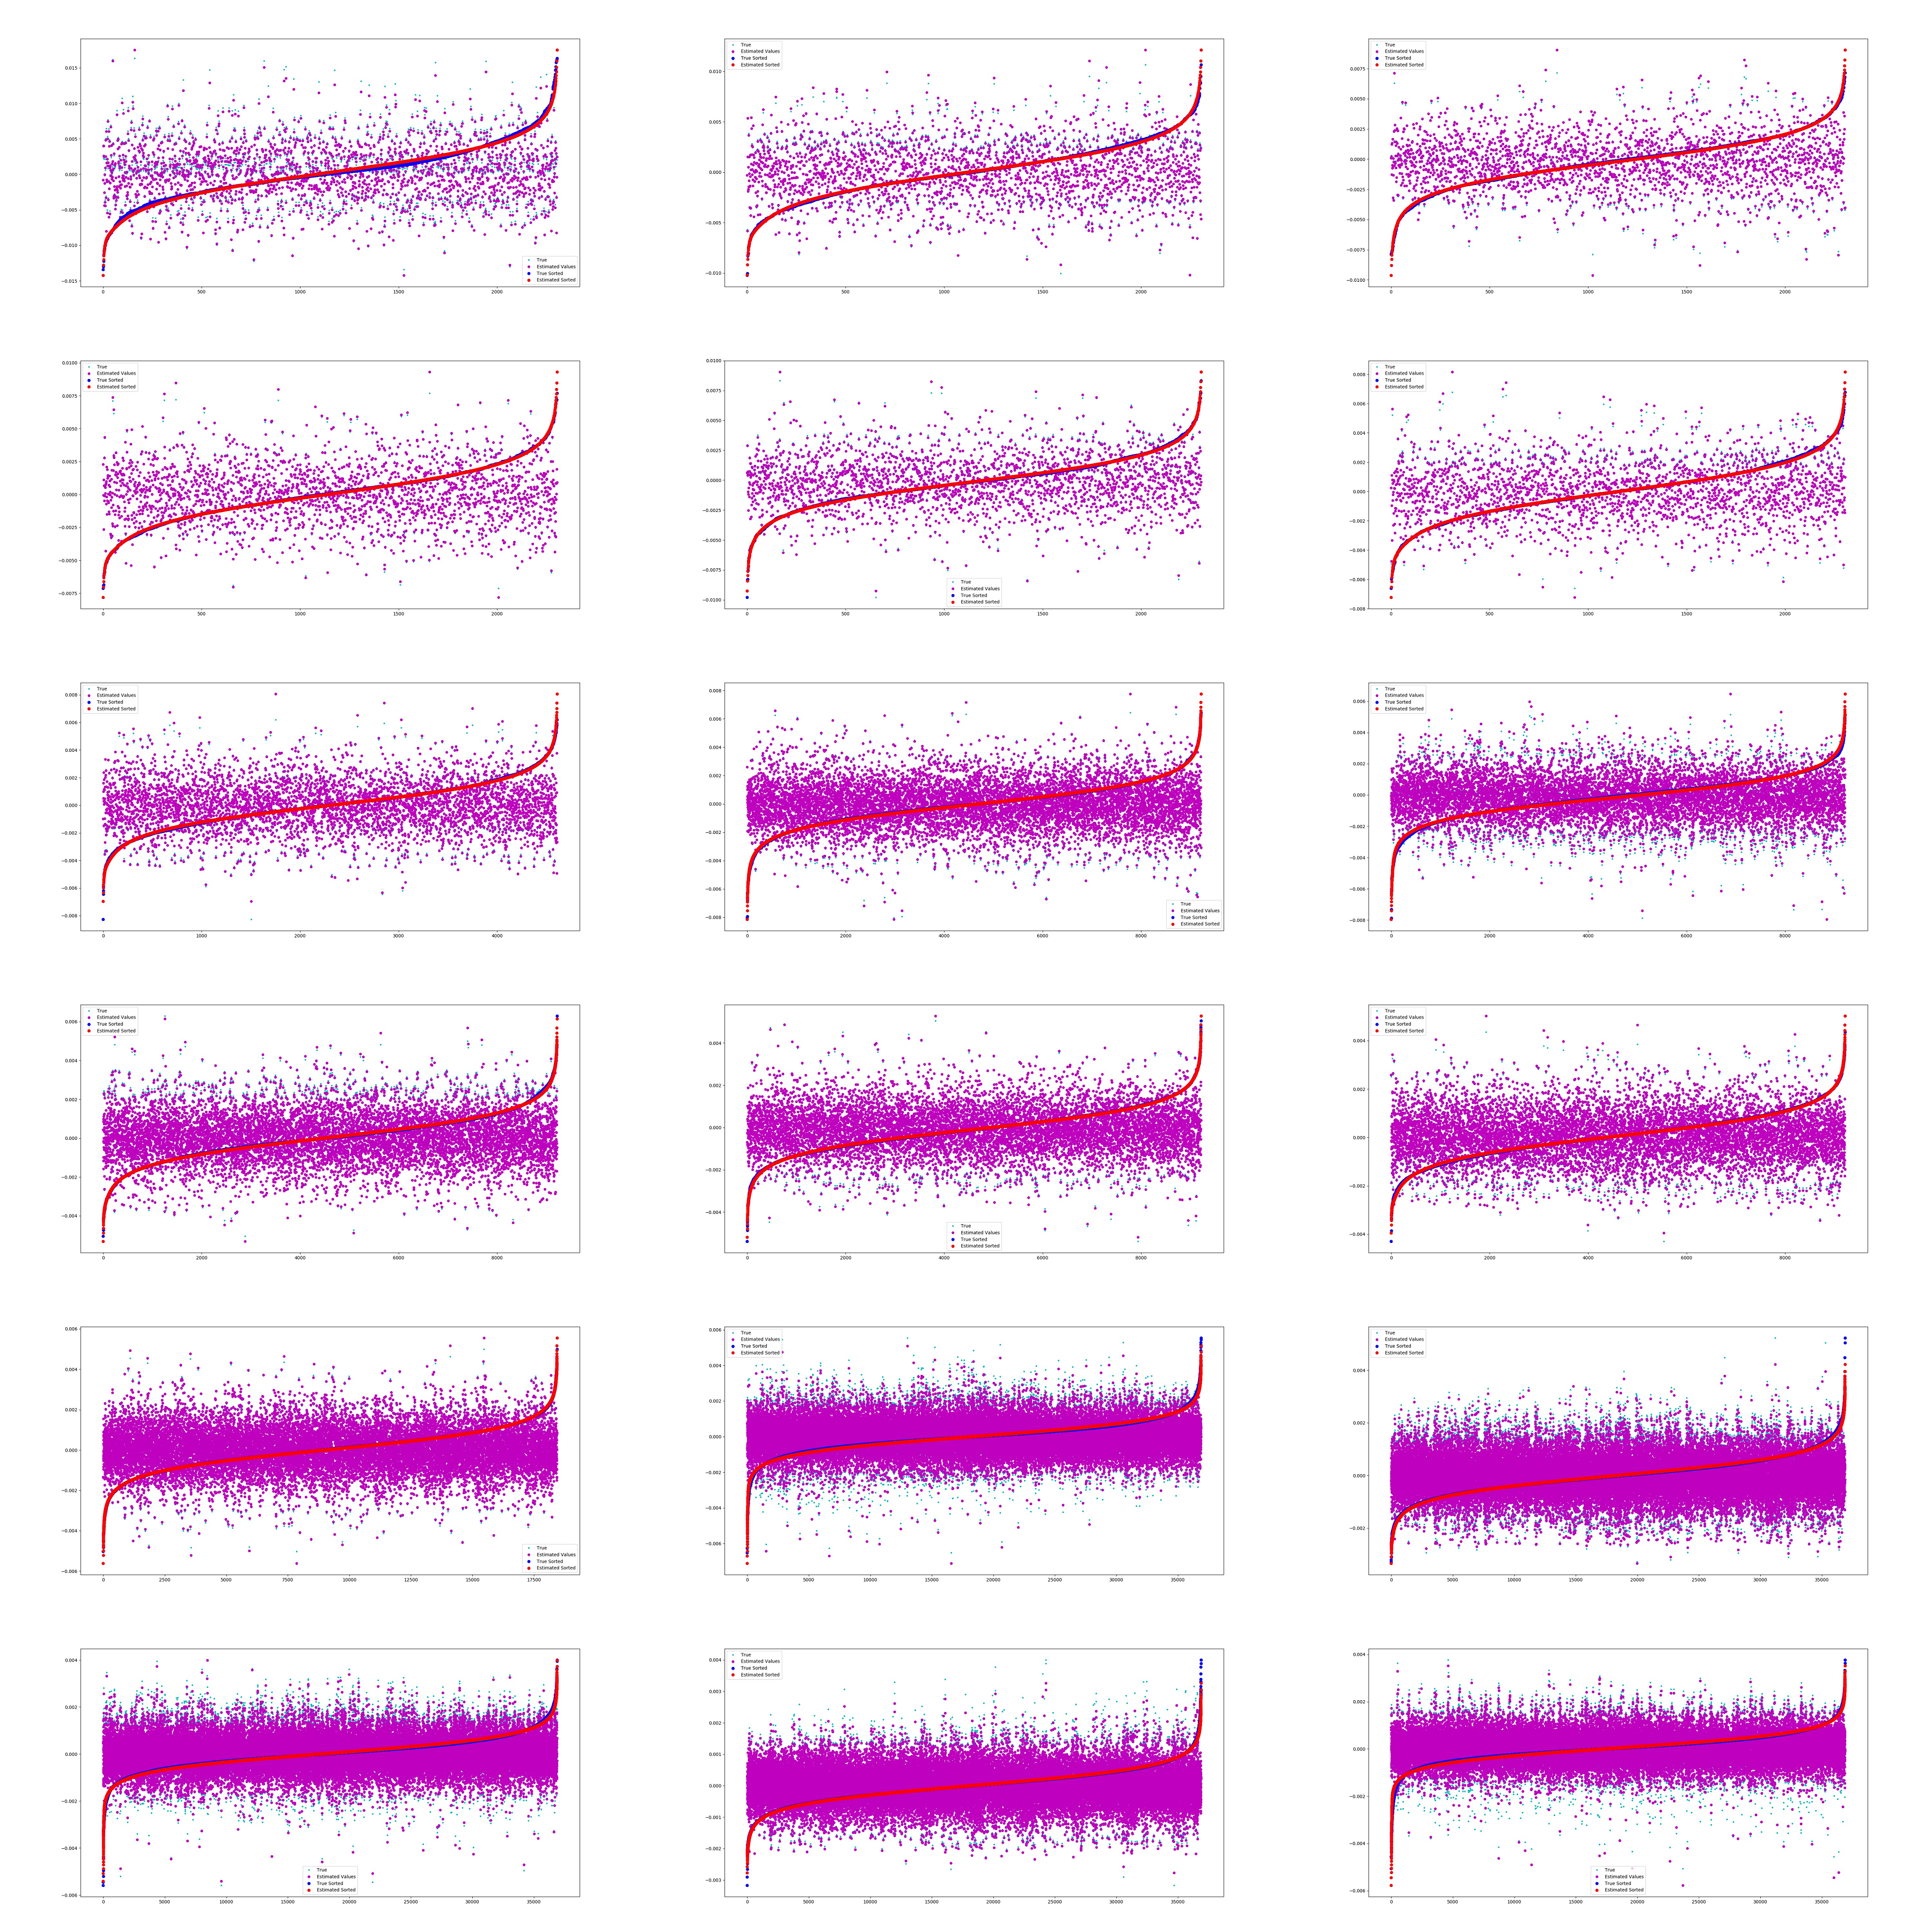
\includegraphics[width=1\textwidth]{thesis/figures/logit_step0 _.png}
\caption{LS regression using logit basis functions}
\medskip
\small
Resnet20 - first step of training - convolutional layers - linear regression using logit basis functions
\label{regressor}
\end{figure}

\newpage

\begin{lstlisting}
# Definition of the Bloom filter operators in tensorflow

using namespace tensorflow;

REGISTER_OP("BloomCompressor")
.Attr("T: {int32, int64, float16, float32, float64}")
.Attr("false_positives_aware: bool")
.Attr("policy: string")
.Attr("hash_num: int")
.Attr("bloom_size: int")
.Attr("bloom_logs_path: string")
.Attr("gradient_id: int")
.Attr("rank: int")
.Attr("verbosity_frequency: int")
.Attr("verbosity: int")
.Input("values: T")
.Input("indices: int32")
.Input("initial_tensor: int32")
.Input("step: int64")
.Output("compressed_tensor: int8")
.Doc(R"doc(Receives the values and the indices, 
           build a bloom filter on the indices 
           and returns the values concatenated with the filter)doc");

REGISTER_OP("BloomDecompressor")
.Attr("policy: string")
.Attr("mem_mode: int")
.Attr("hash_num: int")
.Attr("bloom_size: int")
.Attr("bloom_logs_path: string")
.Attr("gradient_id: int")
.Attr("rank: int")
.Attr("suffix: int")
.Attr("verbosity_frequency: int")
.Attr("verbosity: int")
.Input("compressed_tensor: int8")
.Input("decompressed_size: int32")
.Input("step: int64")
.Output("decompressed_tensor: int32")
.Doc(R"doc(Splits the compressed tensor into 
           values and bloom filter, decodes the indices and 
           returns the re-constructed gradient)doc");

\end{lstlisting}

\end{appendix}
% manually include the bibliography
\bibliographystyle{plain}
\bibliography{references}
% include it also in ToC (do sth on your own)
\addcontentsline{toc}{chapter}{REFERENCES}


\end{document}
